%\addtocontents{toc}{\protect\newpage} % Else toc will break page in the middle
% of the chapter
\chapter{A functional definition of analogical classifiers}
\label{CHAP:functional_definition}
\localtableofcontents*
\vspace*{\baselineskip}

\initial{I}n the previous chapter, we
briefly described a basic process of analogical classification in an informal
way. In this chapter, we will clearly and formally define analogical
classification, which will help us clarify some of the grey areas that we have
glimpsed before. Also (and most
importantly), we will describe our contributions to this problem.

A first form of analogical classifier has been defined in the works of Stroppa
and Yvon \cite{StrYvoCNLL05}, which we will refer to as \textbf{conservative
classifiers}. Another form of analogical classifiers has later been proposed in
the works of Bayoudh, Delhay and Miclet \cite{MicBayDelJAIR08,
BayMicDelIJCAI07}, referred-to here as \textbf{extended classifiers}.

Though the theoretical groundings of the conservative and extended
classifiers have a lot in common (they are both analogical classifiers after
all), we will see that their practical implementations are actually quite
different. We will show however that the extended classifier is a
generalization of the conservative one, and most importantly that these two
approaches can be factorized into a single, unifying framework.

So far, only algorithmic descriptions of both methods were available. Our
unifying framework will allow us to give a general and \textbf{functional}
definition of analogical classifiers, opening the door to some theoretically
grounded research.

This chapter is structured as follows. In Section
\ref{SEC:analogical_classification}, we will review and detail the two previous
approaches to analogical classification, that we will name here the
conservative and the extended classifiers. We will then get to the heart of the
matter and start describing our first contribution, that consists in
factorizing these two approaches into a single functional description. Thanks to
this functional definition of analogical learners\footnote{In what follows, we
will abuse language and use \textit{analogical learner} and
\textit{analogical classifier} as synonyms.}, we will be able in Section
\ref{SEC:theoretical_properties_of_analogical_classifiers} to derive some
theoretical properties about analogical learners. We will indeed show that
their VC-dimension is infinite, and that their accuracy is closely related to
that of the $k$-NN classifier. Finally in Section
\ref{SEC:experiments_and_empirical_validation}, we will empirically verify our
results and provide some insights that will motivate the topic of Chapter
\ref{CHAP:analogy_preserving_functions}.

\section{Analogical classification}
\label{SEC:analogical_classification}

This first section will be devoted to the unification of two seemingly
different analogical approaches to classification.  Let us first define the
problem of classification, one of the main subfields of machine learning. The
aim is simple: a classifier has to estimate the class of any element given as
input on the basis of some other elements for which the class is known.
Formally, we denote $X^m$ our universe which is usually a Cartesian product:
$X^m = X_1 \times X_2 \times \ldots \times X_m$. We have at our disposal a
subset $S \subsetneq X^m \times Y$ of $n$ pairs $\left(\mathbf{x},
f(\mathbf{x})\right)$, called the \textbf{training set}.  $$S=
\Set{\left(\mathbf{x}^{(i)}, f(\mathbf{x}^{(i)})\right) \in X^m \times Y | i
\in [1,n]}.$$

For any $\mathbf{x} \in X^m$, the value $f(\mathbf{x})$ is called its
\textbf{class} or \textbf{label}.
The functional notation $f(\mathbf{x})$ suggests that all labels
are defined by an underlying function $f \colon X^m \to Y$, which is the usual
general view point of machine learning (usually, $\mathbf{x}$ is also
considered as a random variable). In the case of classification, $Y$ is a
finite set of size $C$ where $C$ is the number of different classes. The goal
of a classifier is to \textbf{learn} the function $f$ on the basis of the
elements in $S$, called the \textbf{examples}. The output of a classifier is a
function $\hat{f} \colon X^m \to Y$ that is \textit{as close as possible} the
ground truth function $f$.

\subsection{Conservative classifier}
\label{SEC:conservative_classifier}

We will here describe what we call a \textbf{conservative} classifier. Without
further ado, let us consider Algorithm \ref{ALGO:conservative_classifier} which
describes such classifiers.

\begin{algorithm}[!ht]
\caption{The Conservative classifier.}
\label{ALGO:conservative_classifier}
  \begin{algorithmic}
    \STATE {\bf Input}: A training set $S$ and an element $\mathbf{x} \in X^m
    \setminus S$ for which $f(\mathbf{x})$ is unknown.
    \STATE {\bf Output}: $\hat{f}(\mathbf{x})$, an estimation of
    $f(\mathbf{x})$.
    \STATE {\bf Init}: $\mathbf{C}(\mathbf{x}) = \varnothing$ \quad \quad // A multiset of candidate
    labels.

    \FORALL{$(\mathbf{a}, \mathbf{b}, \mathbf{c}) \in S^3$ such that
    $\mathbf{a} : \mathbf{b} :: \mathbf{c} : \mathbf{x}$}
    \IF{$f(\mathbf{a}) : f(\mathbf{b}) ::f(\mathbf{c}) : y$ is
    solvable}
    \STATE $y = \sol\left(f(\mathbf{a}), f(\mathbf{b}), f(\mathbf{c})\right)$
    \STATE $ \mathbf{C}(\mathbf{x}) = \mathbf{C}(\mathbf{x}) \cup y$
    \ENDIF
	  \ENDFOR
    \STATE $\hat{f}(\mathbf{x}) = \text{Mode} (\mathbf{C}(\mathbf{x}))$ // The most common value in
    $\mathbf{C}(\mathbf{x})$ (undefined if $\mathbf{C}(\mathbf{x}) = \varnothing$).
  \end{algorithmic}
\end{algorithm}

It should be easy to see that the process of Algorithm
\ref{ALGO:conservative_classifier} is extremely similar to the one we followed
on our first introduction to classification with Boolean proportions in
Section \ref{SEC:machine_learning_with_boolean_proportions}. Here again the key
underlying process is the analogical inference principle, which states that if
four elements are in proportion, then their classes should also be in
proportion. But Algorithm \ref{ALGO:conservative_classifier} is slightly more
general than what we have glimpsed in Section
\ref{SEC:machine_learning_with_boolean_proportions}: it allows to deal with
cases where some of the candidate solutions $y$ do not agree with each other.
The fix here is to consider that the prediction $\hat{f}(\mathbf{x})$ will be
the most common candidate solution among all the predictors. This definition of
analogical classification comes from the work of Stroppa and Yvon
\cite{StrYvoCNLL05, StrYvoREPORT05}, and to our knowledge it is the first
instance of analogical learner that has ever been proposed. We note however
that the authors did not explicitly state that the class equations must be
solvable to be useful.

Note that if the multiset $\mathbf{C}(\mathbf{x})$ is empty, i.e. if we cannot find
$3$-tuples in $S^3$ such that they are in proportion with $\mathbf{x}$ and such
that the related class equation is solvable, then the value
$\hat{f}(\mathbf{x})$  is undefined and $\mathbf{x}$ cannot be classified
(hence the name \textit{conservative}).

At first sight, we are here in a setting where the examples in $S$ are stored
for future use, without any generalization process.  We will thus consider (for
now) that the conservative classifier ranges among the category of
\textbf{lazy learners}, i.e. learners that only rely on the training set $S$
without any actual \textit{learning} stage, or without building any model of
the data. The most popular instance of lazy learner certainly is the famous
$k$-NN algorithm.

In the following, we will give a functional definition of $\hat{f}(\mathbf{x})$
as outputted by a conservative classifier. To this end, we will define two
crucial concepts: the \textbf{analogical extension} of a training set $S$, and
the \textbf{analogical root} of an element $\mathbf{x}$. Both the analogical
extension and the analogical root were first defined in \cite{StrYvoREPORT05},
with some minor differences with our definitions.

\begin{definition}[Analogical extension]
  \label{DEF:analogical_extension}
  Denoting $S$ a training set and $f$ the ground truth function of the labels,
  the \textbf{analogical extension} of $S$ using $f$ is:
  $$
  \esf \eqdef \Set{ \mathbf{x} \in X^m |  \exists
  (\mathbf{a},\mathbf{b},\mathbf{c}) \in S^3, ~ \mathbf{a} : \mathbf{b} ::
  \mathbf{c} : \mathbf{x} \text{ and } f(\mathbf{a}) : f(\mathbf{b}) ::
  f(\mathbf{c}) : y \text{ is solvable}}.
  $$
\end{definition}

Intuitively,  $\esf$ can be regarded as the set of all $\mathbf{x} \in X^m$
that are in proportion with at least one 3-tuple in $S$, provided that the
equation related to the associated labels is also solvable. For any $S$ and any
$f$, $\esf$ satisfies some elementary properties:
\begin{enumerate}
\item $S \subseteq \esf$, since $\mathbf{x} : \mathbf{x} :: \mathbf{x}
  :\mathbf{x}$ always holds;
\item $\aext{\varnothing}{f} = \varnothing$, and $\aext{X^m}{f}=X^m$;
\item $S_1 \subseteq S_2 \implies \aext{S_1}{f} \subseteq \aext{S_2}{f}$.
\end{enumerate}
We will denote by $\esfs$ the set of elements in $\esf$ that are not in $S$:
$$\esfs \eqdef \esf \setminus S.$$ In a setting where for any
$\mathbf{a},\mathbf{b}, \mathbf{c}$ the equation $\mathbf{a} : \mathbf{b} ::
\mathbf{c} : \mathbf{x}$ is always solvable (as is the case for the arithmetic
proportion) and such that the associated class equation is also solvable, we
can show that the size of $\esfs$ is exactly $\frac{1}{2} n^2(n - 1)$. This
value is thus a loose upper bound for $\mid \esfs\mid$, because in practice
equations are not always solvable.

\begin{testexample}
To polish our understanding of the analogical extension, let us consider Figure
\ref{FIG:ae_example}.
The training set $S$ is $\Set{\mathbf{a}, \mathbf{b}, \mathbf{d},\mathbf{e}}$.
Taking $(\mathbf{b}, \mathbf{d}, \mathbf{a}) \in S^3$, we notice that
$\mathbf{b} : \mathbf{d} :: \mathbf{a} : \mathbf{c}$, and the associated class
equation $0:1::0:y$ is solvable. So $\mathbf{c}$ is in $\esf$. The same goes for
$\mathbf{f}$ with the 3-tuple $(\mathbf{a}, \mathbf{b}, \mathbf{e}) \in S^3$.
However, even if we can find $(\mathbf{b}, \mathbf{d}, \mathbf{e}) \in S^3$
such that $\mathbf{b} : \mathbf{d} :: \mathbf{e} : \mathbf{g}$, the associated
class equation $0:1::1:y$ is not solvable, so $\mathbf{g} \notin \esf$. At
last, vertex $\mathbf{h}$ will suffer the same fate because the class equation
$f(\mathbf{a}) : f(\mathbf{e}) :: f(\mathbf{d}) : y$ is not solvable either. In
the end, $\esf = \set{\mathbf{a}, \mathbf{b}, \mathbf{c}, \mathbf{d},
\mathbf{e}, \mathbf{f}}$ and $\esfs = \Set{\mathbf{c}, \mathbf{f}}$.
\end{testexample}

\begin{figure}[!h]
\centering
  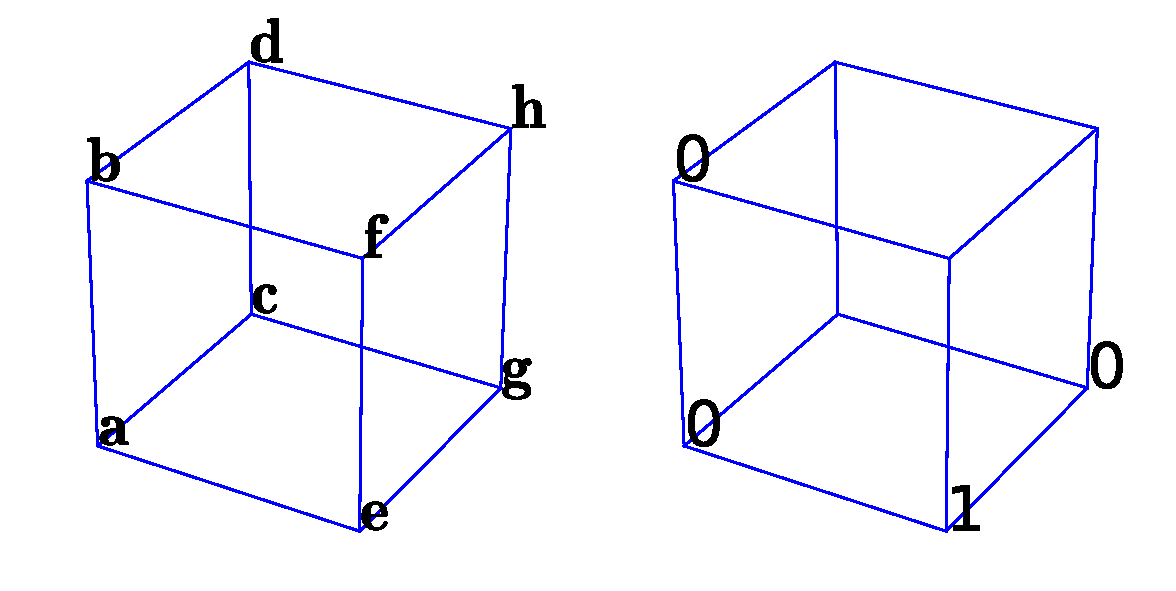
\includegraphics[width=3in]{figures/ae_example.pdf}
  \caption{With $S = \Set{\mathbf{a}, \mathbf{b}, \mathbf{d},
  \mathbf{e}}$, we have $\esfs = \Set{\mathbf{c}, \mathbf{f}}$.}
\label{FIG:ae_example}
\end{figure}

The dual concept of the analogical extension is what we call the
\textbf{analogical root} of a given element $\mathbf{x} \in X^m$:

\begin{definition}[Analogical root]
  \label{DEF:analogical_root}
  Denoting $S$ a training set and $f$ the ground truth function of the labels,
  the \textbf{analogical root} of an element $\mathbf{x} \in X^m$ is:
  $$
  \rsfx \eqdef \Set{(\mathbf{a}, \mathbf{b}, \mathbf{c}) \in S^3 |
  \mathbf{a}:\mathbf{b}::\mathbf{c}:\mathbf{x} \text{ and }
  f(\mathbf{a}):f(\mathbf{b})::f(\mathbf{c}):y \text{ is solvable}}.
  $$
\end{definition}

\noindent
$\rsfx$ is simply the set of 3-tuples in $S$ which are analogically linked to
$\mathbf{x}$.

\begin{testexample}
Considering again the example of Figure \ref{FIG:ae_example}, we have 
$\aroot{S}{f}{\mathbf{c}} = \Set{(\mathbf{b}, \mathbf{d},\mathbf{a}),
(\mathbf{b}, \mathbf{a},\mathbf{d})}$. However, the two corresponding
proportions $\mathbf{b}: \mathbf{d}::\mathbf{a}:\mathbf{c}$ and $\mathbf{b}:
\mathbf{a}::\mathbf{d}:\mathbf{c}$ are equivalent, and we will follow the
convention that the analogical root should only contain non-equivalent
3-tuples, so technically $\aroot{S}{f}{\mathbf{c}}$ is entirely described by
$\Set{(\mathbf{b}, \mathbf{d},\mathbf{a})}$.  We also have 
$\aroot{S}{f}{\mathbf{f}} = \Set{(\mathbf{a}, \mathbf{b},
\mathbf{e})}$, $\aroot{S}{f}{\mathbf{a}} = \Set{(\mathbf{a}, \mathbf{a},
\mathbf{a}), (\mathbf{b}, \mathbf{b}, \mathbf{a}), (\mathbf{d}, \mathbf{d},
\mathbf{a}), (\mathbf{e}, \mathbf{e}, \mathbf{a})}$, and
$\aroot{S}{f}{\mathbf{h}} = \varnothing$. \end{testexample}

It is clear that in general, $$\rsfx = \varnothing\iff \mathbf{x} \notin
\esf.$$ It should also be clear that even if we only consider unique 3-tuples
(up to equivalence) in the analogical root, $\rsfx$ may contain more than one
3-tuple: for example in $\mathbb{R}^m$ or $\mathbb{B}^m$ with the arithmetic
(or Boolean) proportion, $\mathbf{x}$ may be the involved in more than one
parallelogram, as illustrated in Figure \ref{FIG:multiple_parallelograms}.

\begin{figure}[!h]
\centering
  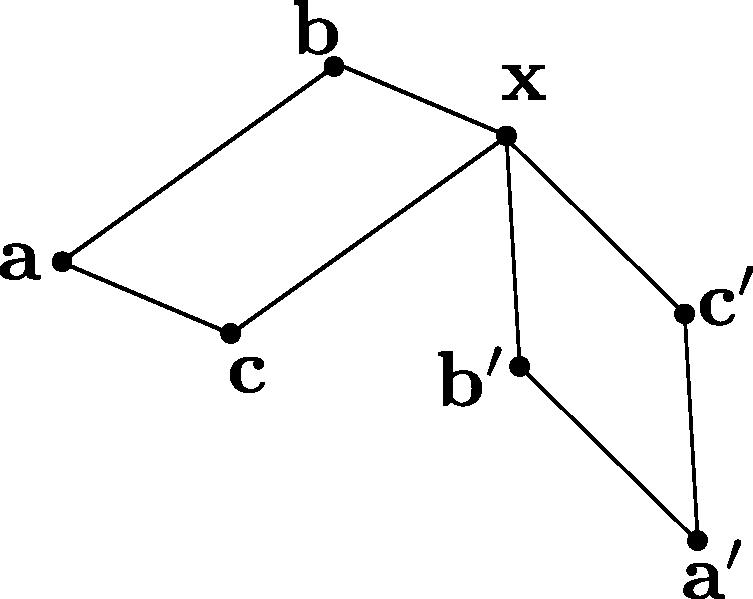
\includegraphics[width=2.5in]{figures/multiple_parallelograms.pdf}
  \caption{With $S = \Set{\mathbf{a}, \mathbf{b}, \mathbf{c}, \mathbf{a}',
  \mathbf{b}', \mathbf{c}'}$, we have $\mathbf{x} \in \esf$ and $\rsfx =
  \Set{(\mathbf{a}, \mathbf{b}, \mathbf{c}), (\mathbf{a}', \mathbf{b}',
  \mathbf{c}')}$. Class equations are all assumed to be solvable.}
\label{FIG:multiple_parallelograms}
\end{figure}

We need to introduce one last definition before we can go on with the
functional view of conservative classifiers:

\begin{definition}[Analogical label]
  \label{DEF:analogical_label}
  For any element $\mathbf{x}$ of $\esf$, we denote $\mathbf{C}(\mathbf{x})$
  the set of solutions to the class equations associated with $\mathbf{x}$:
  $$\mathbf{C}(\mathbf{x}) \eqdef \Set{y | f(\mathbf{a}) : f(\mathbf{b}) ::
  f(\mathbf{c}) :y, \quad \text{with }(\mathbf{a}, \mathbf{b}, \mathbf{c}) \in \rsfx}$$
  We then define the \textbf{analogical
  label} of $\mathbf{x}$, denoted $\albl{\mathbf{x}}$, as:
  $$\albl{\mathbf{x}} \eqdef
  \begin{cases}
    f(\mathbf{x}) \text{ if } \mathbf{x} \in S\\
    \text{Mode} \left(\mathbf{C}(\mathbf{x})\right) \text{ if
    } x \notin S
  \end{cases}
  $$
  where $\text{Mode}(\mathbf{C})$ returns the most frequent element of the multiset
$\mathbf{C}$. In case of a tie, the returned element is chosen at random between
the most frequent elements.
\end{definition}

\noindent
We are now in position to give a functional definition of the conservative
classifier:

\begin{definition}[Conservative classifier]
  \label{DEF:conservative_classifier}
  Given a training set $S$ with an underlying ground truth function $f$,
  a \textbf{conservative classifier} sets the prediction of an element $\mathbf{x}$ as
  follows:

  $$\text{If } \mathbf{x} \in \esf, ~ \hat{f}(\mathbf{x}) \eqdef \albl{\mathbf{x}}.
  \text{ Else, } \hat{f}(\mathbf{x}) \text{ is undefined.}$$
\end{definition}

As previously mentioned, a conservative classifier is not able to output a
prediction if $\mathbf{x}$ does not belong to the analogical extension. We have
already made this observation when describing Algorithm
\ref{ALGO:conservative_classifier}: for a given $\mathbf{x}$, the set of
candidate solutions $\mathbf{C}(\mathbf{x})$ is empty if and only if
$\mathbf{x} \notin \esf$.  Also, we now understand why $\albl{\mathbf{x}}$ is
simply set to $f(\mathbf{x})$ when the $\mathbf{x} \in S$: for such an
$\mathbf{x}$ it is natural to want $\hat{f}(\mathbf{x}) = f(\mathbf{x})$!

\begin{testexample}
Going
back to our example with Figure \ref{FIG:ae_example}, we will have
$\hat{f}(\mathbf{c}) \eqdef \albl{\mathbf{c}} = 1$, because
$\aroot{S}{f}{\mathbf{c}} = \Set{(\mathbf{b}, \mathbf{d},\mathbf{a})}$ and
$\mathbf{C}(\mathbf{c}) = \Set{1}$. Also, $\hat{f}(\mathbf{f}) \eqdef
\albl{\mathbf{f}} = 1$, because $\aroot{S}{f}{\mathbf{f}} =
\Set{(\mathbf{a},\mathbf{b},\mathbf{e})}$ and $\mathbf{C}(\mathbf{f}) =
\Set{1}$. Here, we did not need to use the majority-vote procedure as there was
only one candidate solution for each prediction. As $\mathbf{g}$ and
$\mathbf{h}$ do not belong to $\esf$, both $\albl{\mathbf{g}}$ and
$\albl{\mathbf{h}}$ stay undefined.
\end{testexample}

Let us note that in Algorithm \ref{ALGO:conservative_classifier}, the
analogical extension $\esf$ is never explicitly computed. Instead, for a given
$\mathbf{x}$, we look for
every 3-tuple in $S^3$ and check if they belong to $\rsfx$. One drawback is
that the search in $S^3$ has to be done for every new element $\mathbf{x}$ that
we want to classify, and can prove to be quite expensive in computation time,
even for small sizes of $S$. However, taking advantage of our functional
definition, we can reformulate the learning process of a conservative
classifier as follows:

\begin{itemize}
\item First, compute $\esf$. While $\esf$ is begin computed, it is trivial to
  also compute the set of candidates $\mathbf{C}(\mathbf{x})$ for each $x \in
    \esf$.
  \item Then, for all $x \in\esf$, compute
    $\albl{\mathbf{x}} \eqdef \text{Mode}(\mathbf{C}(\mathbf{x}))$.
\end{itemize}
\noindent
Whenever we are asked to classify a given $\mathbf{x}$, all we need now is to
check whether $\mathbf{x}$ belongs to $\esf$ or not. The output
$\hat{f}(\mathbf{x})$ is then immediate. This way to proceed has the undeniable
advantage to perform the search in $S^3$ only once. Obviously, this saving in
computation time is done at the expense of memory consumption, because the
size of $\esf$ can be drastically greater than that of $S$. This alternative
view also leads us to reconsider our previous statement about conservative
classifiers belonging to the class of lazy learners. Here, the computation of
the analogical extension can be viewed as a generalization process, even if not
all elements of the universe $X^m$ are affected by this generalization.

We will end this discussion on conservative classifier by sketching a use-case
described in \cite{StrYvoREPORT05}, where an analogical proportion is defined
on the set of words over a finite alphabet, and the task is to learn the
conjugation of English verbs. This setting is slightly different from that of
classification that we have settled-in, but all definitions and concepts remain
valid. Here, solving the analogical equation
$\textit{view}:\textit{reviewer}::\textit{search}:y$ leads to $\textit{researcher}$,
using the definition of the analogy and the concatenation operator.


\begin{testexample}
We have a training set $S=\Set{\mathbf{x}^{(1)},\mathbf{x}^{(2)},
\mathbf{x}^{(3)}, \mathbf{x}^{(4)}, \mathbf{x}^{(5)}}$ where
  $\mathbf{x}^{(1)}=(\textit{read},3,\textit{reads}),
  \mathbf{x}^{(2)}=(\textit{read},G,\textit{reading}),
  \mathbf{x}^{(3)}=(\textit{view},3,\textit{views})$,
  $\mathbf{x}^{(4)}=(\textit{view},G,\textit{viewing}),
  \mathbf{x}^{(5)}=(\textit{eat},3,\textit{eats})$.\\
  $(\textit{read},3,\textit{reads})$ means that $\textit{read}$ is
  transformed into $\textit{reads}$ when conjugated at the third person
  singular, and $G$ stands for the gerund form.

  Given a new element $\mathbf{x}=(\textit{eat},G,?)$, $\rsfx=
\Set{\left(\mathbf{x}^{(1)}, \mathbf{x}^{(2)}, \mathbf{x}^{(5)}\right),
\left(\mathbf{x}^{(3)},\mathbf{x}^{(4)},\mathbf{x}^{(5)}\right)}$. The
prediction is as expected $\hat{f}(\mathbf{x})=\textit{eating}$, which is the
solution of the equations $\textit{reads}:\textit{reading}::\textit{eats}:y$ and
$\textit{views}:\textit{viewing}::\textit{eats}:y$. There is
  no solution for $\mathbf{x}=(\textit{absurd},G,y)$, just because $\rsfx=
  \varnothing$.
\end{testexample}

The fact that conservative learners cannot output a prediction for any
$\mathbf{x}$ can here be considered a good thing: it would not be natural to
look for the gerund form of \textit{absurd}. However, in many use-cases we do
want our classifier to be able to predict the label of any element. This is why
other options have been implemented to overcome this problem, and to extend in
some sense the generalization ability of analogical learners. This is the
purpose of \textbf{extended classifiers} described in the next section.

\subsection{Extended classifier}
\label{SEC:extended_classifier}

We now want our analogical classifier to be able to predict the label of any
input element $\mathbf{x} \in X^m$, and not just the ones in $\esf$.
The main bottleneck of Algorithm \ref{ALGO:conservative_classifier} is that we
require the 3-tuples in $S^3$ to be in perfect proportion with the element
$\mathbf{x}$ we want to classify. Such 3-tuples are not always available in the
training set, so necessarily some elements of $X^m$ are excluded from $\esf$.

The key concept that will help us overcome this issue is what we call an
\textbf{analogical dissimilarity}, first introduced in
\cite{BayMicDelIJCAI07}. The analogical dissimilarity is a measure that
quantifies in some sense \textit{how far} a relation $\mathbf{a} : \mathbf{b}
:: \mathbf{c} : \mathbf{d}$ is from being a perfectly valid proportion.

We keep the initial notation $\AD(\mathbf{a}, \mathbf{b},
\mathbf{c},\mathbf{d})$ to denote the analogical dissimilarity between 4
elements.  Some  minimal properties have to be satisfied by such a
dissimilarity $\AD \colon {(X^m)}^4 \longrightarrow \mathbb{R}^+$ to fit
with the intuition. For any $\mathbf{a}, \mathbf{b},\mathbf{c},\mathbf{d},
\mathbf{e}, \mathbf{f} \in X^m$, the following properties should hold:
\begin{itemize}
  \item $\AD(\mathbf{a}, \mathbf{b},\mathbf{c},\mathbf{d})=0 \iff \mathbf{a} :
    \mathbf{b}:: \mathbf{c} : \mathbf{d}$ (Consistency with the Analogy)
  \item $\AD(\mathbf{a}, \mathbf{b},\mathbf{c},\mathbf{d})=
    \AD(\mathbf{c}, \mathbf{d},\mathbf{a},\mathbf{b})$ (Symmetry)
  \item $\AD(\mathbf{a}, \mathbf{b},\mathbf{c},\mathbf{d})=
    \AD(\mathbf{a}, \mathbf{c},\mathbf{b},\mathbf{d})$ (Central permutation)
  \item $\AD(\mathbf{a}, \mathbf{b},\mathbf{e},\mathbf{f}) \leq \AD(\mathbf{a},
    \mathbf{b},\mathbf{c},\mathbf{d}) + \AD(\mathbf{c},
    \mathbf{d},\mathbf{e},\mathbf{f})$ (Triangle inequality)
  \item In general, $\AD(\mathbf{a}, \mathbf{b},\mathbf{c},\mathbf{d}) \neq
    \AD(\mathbf{b}, \mathbf{a},\mathbf{c},\mathbf{d})$
\end{itemize}
Naturally, the symmetry and central permutation properties lead to the same
three classes of equivalence that we have for the analogical proportion. In
particular, the equivalence class that is \textit{generated} by
$\AD(\mathbf{a}, \mathbf{b},\mathbf{c},\mathbf{d})$ is:
\begin{align*}
  &\AD(\mathbf{a}, \mathbf{b},\mathbf{c},\mathbf{d}) =
\AD(\mathbf{c}, \mathbf{d},\mathbf{a},\mathbf{b})=
\AD(\mathbf{c}, \mathbf{a},\mathbf{d},\mathbf{b})=
\AD(\mathbf{d}, \mathbf{b},\mathbf{c},\mathbf{a})=
\AD(\mathbf{d}, \mathbf{c},\mathbf{b},\mathbf{a})=\\
  &\AD(\mathbf{b}, \mathbf{a},\mathbf{d},\mathbf{c})=
\AD(\mathbf{b}, \mathbf{d},\mathbf{a},\mathbf{c})=
\AD(\mathbf{a}, \mathbf{c},\mathbf{b},\mathbf{d}).
\end{align*}

The definition of an analogical proportion strongly relies on the structure and
operators available on $X^m$, and the same goes for the definition of the
analogical dissimilarity: there are a lot of possibilities. For the arithmetic
proportion in $\mathbb{R}^m$, the analogical dissimilarity  $\AD(\mathbf{a},
\mathbf{b},\mathbf{c},\mathbf{d})$ should capture \textit{how far}
are $\mathbf{a}, \mathbf{b},\mathbf{c},\mathbf{d}$ from making up a perfect
parallelogram. This can be achieved using the following definition:

% Note: leave \emph{AD} here else it will be in italics.
\begin{definition}[Analogical dissimilarity for real vectors]
  \label{DEF:AD_arithmetic_proportion}
  Given four vectors $\mathbf{a}, \mathbf{b},\mathbf{c},\mathbf{d}$ of
  $\mathbb{R}^m$ equipped with the standard $p$-norm $\norm{p}{\cdot}$, the
  analogical dissimilarity related to the arithmetic proportion is defined as:
  $$\text{AD}(\mathbf{a}, \mathbf{b},\mathbf{c},\mathbf{d}) =
  \norm{p}{(\mathbf{a} - \mathbf{b}) - (\mathbf{c} - \mathbf{d})}.$$
\end{definition}

Of course, we will need an analogical dissimilarity in $\mathbb{B}^m$, but we
will start small and consider $\mathbb{B}$ first:
\begin{definition}[Analogical dissimilarity for Boolean vectors]
  \label{DEF:AD_boolean_proportion}
  Given four elements $a, b, c, d$ of $\mathbb{B}$, the analogical
  dissimilarity $\text{AD}(a, b, c, d)$ is defined as the number of values that
  have to be switched to get a proper analogy.
\end{definition}
\noindent
Table \ref{TAB:analogical_dissimilarity} shows the values of $\AD(a, b, c, d)$
for 8 patterns. The $8$ remaining patterns have the same values of $AD$ as
their negated versions and have thus been ignored.
\begin{table}[t]
  \centering
  $$
  \begin{array}{ccccc}
    \toprule
    a & b & c & d &  \AD(a, b, c, d)\\
    \midrule
    0 & 0 & 0 & 0 &   \textbf{0}\\
    0 & 1 & 0 & 1 &   \textbf{0}\\
    0 & 0 & 1 & 1 &   \textbf{0}\\
    0 & 0 & 0 & 1 &   \textbf{1}\\
    0 & 0 & 1 & 0 &   \textbf{1}\\
    0 & 1 & 0 & 0 &   \textbf{1}\\
    1 & 0 & 0 & 0 &   \textbf{1}\\
    0 & 1 & 1 & 0 &   \textbf{2}\\
    \bottomrule
  \end{array}
  $$
  \caption{The values of $\text{AD}(a, b, c,d)$ for $8$ patterns of $a, b, c,
  d$ in $\mathbb{B}$. The $8$ remaining patterns are the negated versions of
  these.}
  \label{TAB:analogical_dissimilarity}
\end{table}
The natural extension to $\mathbb{B}^m$ is again to consider component-wise
proportions. The analogical dissimilarity in $\mathbb{B}^m$ is thus defined as
the sum of the $m$ individual ADs:
$$\AD(\mathbf{a}, \mathbf{b},\mathbf{c},\mathbf{d}) = \sum\limits_{i=1}^m
\AD(a_i,b_i,c_i,d_i).$$
We get an analogical dissimilarity whose co-domain is $[0, 2m]$. In fact, if we
use the $1$-norm defined as $\norm{1}{\mathbf{x}} = \sum_{i = 1}^m |x_i|$,
Definition \ref{DEF:AD_arithmetic_proportion} is equivalent to Definition
\ref{DEF:AD_boolean_proportion}. This means that for $\mathbf{a},
\mathbf{b},\mathbf{c},\mathbf{d}$ in $\mathbb{B}^m$, $\AD(\mathbf{a},
\mathbf{b},\mathbf{c},\mathbf{d}) =
\norm{1}{(\mathbf{a}-\mathbf{b})-(\mathbf{c}-\mathbf{d})}$. Note that the
expression $\norm{1}{(\mathbf{a}-\mathbf{b})-(\mathbf{c}-\mathbf{d})}$ is
nothing but the Hamming distance between the two vectors\footnote{$\mathbb{B}^m$
is not closed under addition (or subtraction), so technically it may happen that
$(\mathbf{a} - \mathbf{b}), (\mathbf{c} - \mathbf{d})$, or their difference are
not in $\mathbb{B}^m$ but in $\mathbb{R}^m$.}
$(\mathbf{a}-\mathbf{b})$ and $(\mathbf{c}-\mathbf{d})$.
Actually, we could use any $p$-norm in $\mathbb{B}^m$, so
Definition \ref{DEF:AD_arithmetic_proportion} could also be used to give a more
general definition of the analogical dissimilarity in $\mathbb{B}^m$. Here
again, we are witnessing the close bond that links the Boolean proportion and
and the arithmetic proportion.

As a measure of \textit{how poorly an analogical proportion holds}, the
analogical dissimilarity will help us to define more flexible classifiers.  The
main underlying idea is to consider {\it approximate} analogies which are not
valid stricto sensu, but not too far to be valid.
In \cite{BayMicDelIJCAI07}, after defining analogical dissimilarity,  the authors
build an extended classifier allowing classification of elements that do not
belong to $\esf$. Algorithm \ref{ALGO:extended_classifier} gives a
description of their classifier.

\begin{algorithm}[!ht]
 \caption{The extended classifier.}
       \label{ALGO:extended_classifier}
       \begin{algorithmic}

      \STATE {\bf Input}: A training set $S$, an element $\mathbf{x} \in X^m$
         for which $f(\mathbf{x})$ is unknown, and a constant $k > 0$.
         \STATE {\bf Output}: $\hat{f}(\mathbf{x})$, an estimation of
         $f(\mathbf{x})$.
    \STATE {\bf Init}: $\mathbf{C}(\mathbf{x}) = \varnothing$ \quad \quad // A
    multiset of candidate labels.
    \FORALL{$(\mathbf{a}, \mathbf{b}, \mathbf{c}) \in S^3$ such that
         $f(\mathbf{a}) : f(\mathbf{b}) :: f(\mathbf{c}) : y$ is solvable}
         \STATE compute $\AD(\mathbf{a}, \mathbf{b}, \mathbf{c}, \mathbf{x})$ and store it
	    \ENDFOR
         \FORALL{$k$ least values of $\AD(\mathbf{a}, \mathbf{b}, \mathbf{c}, \mathbf{x})$}
        \STATE $y = \sol\left(f(\mathbf{a}), f(\mathbf{b}), f(\mathbf{c})\right)$
    \STATE $ \mathbf{C}(\mathbf{x}) = \mathbf{C}(\mathbf{x}) \cup y$
    \ENDFOR
    \STATE $\hat{f}(\mathbf{x}) = \text{Mode} (\mathbf{C}(\mathbf{x}))$ // The
         most common value in $\mathbf{C}(\mathbf{x})$
\end{algorithmic}
\end{algorithm}


This algorithm is similar to the conservative one, but instead of looking for
pure, flawless proportions, we allow for some analogies not to be perfect when
we need to. This translates into the fact that we now only
look for $3$-tuples in $S^3$ such that the class equation is solvable. We do
not care if they are in perfect proportion with $\mathbf{x}$. Such
$3$-tuples \textbf{always} exist in $S^3$, simply because we can choose any
$3$-tuple $(\mathbf{a}, \mathbf{a}, \mathbf{a})$ with $\mathbf{a} \in S$.
Hence, Algorithm \ref{ALGO:extended_classifier} is able to predict the label of
any element $\mathbf{x} \in X^m$.

For the sake of simplicity, we ignored here a small but relevant detail:
in their implementation \cite{BayMicDelIJCAI07}, the authors actually look for
all the 3-tuples that have the same analogical dissimilarity as the
$k^\text{th}$ one. For example if the $k^\text{th}$ 3-tuple has an $\AD$ of 5,
they will actually consider all the $3$-tuples that have an $\AD$ less than or
equal to $5$, bringing the number of candidates to $k'$ with $k' \geq k$. This
is fortunate because it allows their extended classifier to
fit with the previous conservative approach in the case of a perfect
proportion (or equivalently, in the case where $\mathbf{x} \in \esf$).  Indeed,
when the $k^\text{th}$ $3$-tuple $(\mathbf{a}, \mathbf{b}, \mathbf{c})$ has an
$\AD$ of $0$, i.e. $\mathbf{a} : \mathbf{b} :: \mathbf{c} : \mathbf{x}$ stands,
they will consider all other $3$-tuples $(\mathbf{a}',
\mathbf{b}',\mathbf{c}')$ such that $\mathbf{a}' : \mathbf{b}' :: \mathbf{c}' :
\mathbf{x}$, which is consistent with the conservative approach. Clearly, the
extended classifier is a generalization of the conservative one.

\begin{testexample}
To better grasp the behaviour of the extended classifier, we will consider
again Figure \ref{FIG:ae_example} that we repeat here for the sake of
  convenience on page \pageref{FIG:ae_example2}. Let us go
through the classification process of $\mathbf{c}, \mathbf{f}, \mathbf{g}$ and
$\mathbf{h}$. We will here consider $k$ to be equal to $1$. For $\mathbf{c}$,
the $3$-tuple in $S^3$ with the least value of $\AD$ is $(\mathbf{b},
\mathbf{d}, \mathbf{a})$ with $\AD(\mathbf{b},\mathbf{d}, \mathbf{a},
\mathbf{c}) = 0$. The set $\mathbf{C}(\mathbf{c})$ is thus $\Set{1}$, and leads
to the prediction $\hat{f}(\mathbf{c}) = 1$. For $\mathbf{f}$, the best
$3$-tuple is $(\mathbf{a}, \mathbf{b}, \mathbf{e})$ and leads to the prediction
$\hat{f}(\mathbf{f}) = 1$. For these two elements in $\esf$, the extended
classifier outputs the same predictions as the conservative one, and most
  importantly, the underlying process is the same (to some extent, this
  is due to the fact that we have chosen $k = 1$).

Consider now $\mathbf{g} \notin \esf$. We know that we won't find any $3$-tuple
in perfect proportion with $\mathbf{g}$ (else the conservative classifier would
have been able to output $\hat{f}(\mathbf{g})$), but the $3$-tuple
$(\mathbf{e}, \mathbf{e}, \mathbf{e}) \in S^3$ has $\AD(\mathbf{e}, \mathbf{e},
\mathbf{e}, \mathbf{c}) = 1$. We have $k = 1$, so strictly following Algorithm
\ref{ALGO:extended_classifier} would lead us to stick to this only $3$-tuple.
However, considering the above remark we are allowed to look for all other
$3$-tuples that also have an $\AD$ of $1$. Actually, the $3$-tuple
$(\mathbf{b}, \mathbf{d}, \mathbf{a})$ also has $\AD(\mathbf{b},\mathbf{d},
\mathbf{a}, \mathbf{g}) = 1$, as can be verified on table \ref{TAB:AD_bdag}. We
thus have $\mathbf{C}(\mathbf{g}) = \Set{1, 1}$: one solution comes from the
  solving of
$f(\mathbf{e)} :f(\mathbf{e}):: f(\mathbf{e}) : y$ and the other solution 
comes from the solving of $f(\mathbf{b)} :f(\mathbf{d}):: f(\mathbf{a}) : y$.  Finally, we
have $\hat{f}(\mathbf{g}) = 1$. As for $\mathbf{h}$, we have
$\mathbf{C}(\mathbf{h}) = \Set{1, 1}$: one solution comes from $f(\mathbf{a)}
:f(\mathbf{b}):: f(\mathbf{e}) : y$ and the other comes from $f(\mathbf{d)}
:f(\mathbf{d}):: f(\mathbf{d}) : y$, and we end up with $\hat{f}(\mathbf{h}) =
1$.
\end{testexample}

\begin{figure}[!h]
\centering
  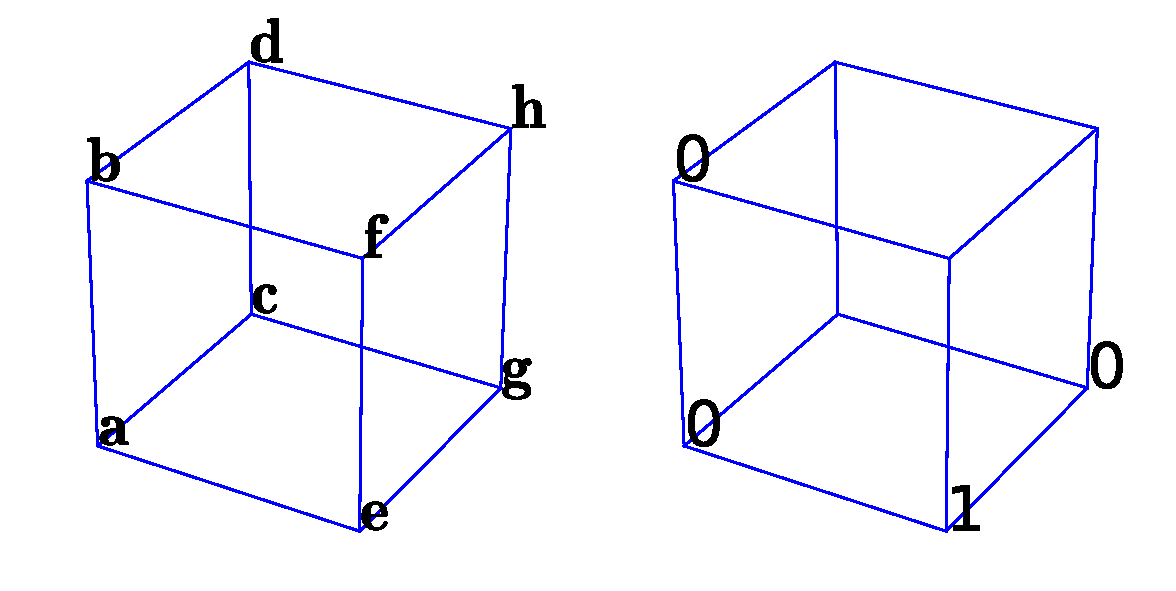
\includegraphics[width=3in]{figures/ae_example.pdf}
  \repeatcaption{FIG:ae_example}{With $S = \Set{\mathbf{a}, \mathbf{b}, \mathbf{d},
  \mathbf{e}}$, we have $\esfs = \Set{\mathbf{c}, \mathbf{f}}$.}
  \label{FIG:ae_example2}
\end{figure}

\begin{table}[t]
  \centering
  $$
  \begin{array}{ccccc}
    \toprule
    \mathbf{b} & \mathbf{d} & \mathbf{a} & \mathbf{g} &  \AD(b_i, d_i, a_i, g_i)\\
    \midrule
    0 & 0 & 0 & 1 &   \textbf{1}\\
    0 & 1 & 0 & 1 &   \textbf{0}\\
    1 & 1 & 0 & 0 &   \textbf{0}\\
    \bottomrule
  \end{array}
  $$
  \caption{$\AD(\mathbf{b}, \mathbf{d}, \mathbf{a}, \mathbf{g}) = 1$.}
  \label{TAB:AD_bdag}
\end{table}



In \cite{BayMicDelIJCAI07}, the authors evaluated this classifier on a Boolean
setting $\mathbb{B}^m$ over 8 benchmarks from the UCI repository.  This
approach led to remarkable results in terms of accuracy, when compared to
off-the-shelf standard classifiers. Nonetheless, this algorithmic description
of the extended classifier does not allow us to grasp its inherent working
behaviour, and it is difficult to extract theoretical properties. The aim of
the next subsection is to give a functional translation of this algorithmic
description.

\subsection{Analogical classifier: a functional definition}
\label{SEC:functional_definition}

As we have previously seen, we can generally assume that
$\AD(\mathbf{a},\mathbf{b},\mathbf{c},\mathbf{d}) \eqdef
\norm{p}{(\mathbf{a}-\mathbf{b})-(\mathbf{c}-\mathbf{d})}$, whether we are
dealing with the arithmetic proportion or the Boolean proportion.
A key observation is that we can formulate this expression with a distance
function on $X^m$. Indeed, a simple rewriting leads to the following expression:
$$\AD(\mathbf{a},\mathbf{b},\mathbf{c},\mathbf{d})=\norm{p}{\mathbf{d} -
(\mathbf{c}-\mathbf{a}+\mathbf{b})}=\norm{p}{\mathbf{d} - \mathbf{d}'},$$
where $\mathbf{d}'\eqdef\mathbf{c}-\mathbf{a}+\mathbf{b}$. Actually,
$\mathbf{d}'$ is nothing but the $4^\text{th}$ vertex of the parallelogram
$\mathbf{a}\mathbf{b}\mathbf{c}\mathbf{d}'$, or equivalently, $\mathbf{d}'$ is
the
solution of the equation $\mathbf{a}: \mathbf{b} :: \mathbf{c} : \mathbf{x}$.
All this means that $\AD(\mathbf{a},\mathbf{b},\mathbf{c},\mathbf{d})$ simply
is the distance between $\mathbf{d}$ and this $4^\text{th}$ vertex
$\mathbf{d}'$: $\AD(\mathbf{a},\mathbf{b},\mathbf{c},\mathbf{d}) =
\delta_p(\mathbf{d}, \mathbf{d}')$, where $\delta_p$ is the distance defined by
the $p$-norm. Figure \ref{FIG:analogical_dissimilarity} schematically sums up all the aforementioned
properties.  Note that when $(\mathbf{a}, \mathbf{b}, \mathbf{c}) \in S^3$ and
when the associated class equation is solvable, we naturally have $\mathbf{d}'
\in \esf$.
\begin{figure}[!h]
\centering
  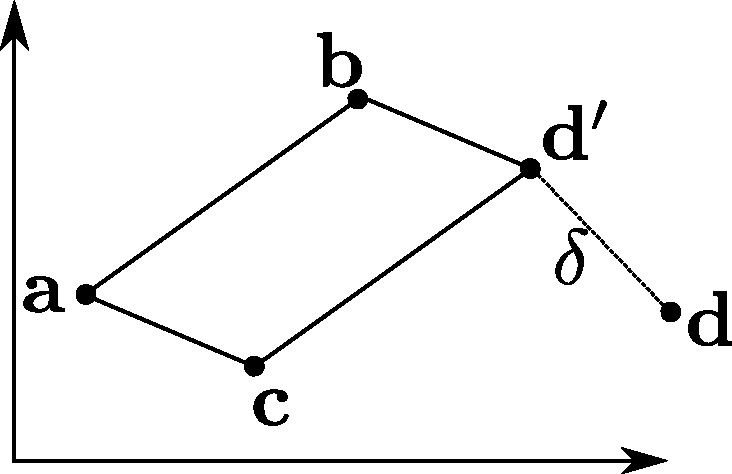
\includegraphics[width=2.5in]{figures/analogical_dissimilarity.pdf}
  \caption{The analogical dissimilarity
  $\AD(\mathbf{a},\mathbf{b},\mathbf{c},\mathbf{d})$ is equal to the distance
  $\delta(\mathbf{d}, \mathbf{d}')$.}
\label{FIG:analogical_dissimilarity}
\end{figure}

\begin{testexample}
Let us consider (again) Figure \ref{FIG:ae_example} on page
\pageref{FIG:ae_example2}. We have already seen that $\AD(\mathbf{b},
\mathbf{d}, \mathbf{a}, \mathbf{g}) = 1$, as proved by Table \ref{TAB:AD_bdag}
  on page \pageref{TAB:AD_bdag}.
We now can reinterpret this statement: $\AD(\mathbf{b}, \mathbf{d}, \mathbf{a},
\mathbf{g})$ should be equal to the distance between $\mathbf{g}$ and another
vector that makes up a perfect parallelogram with the $3$-tuple
$(\mathbf{b},\mathbf{d}, \mathbf{a})$. This vector is naturally
$\sol(\mathbf{b},\mathbf{d}, \mathbf{a}) = \mathbf{c}$ and have indeed
$H(\mathbf{c}, \mathbf{g}) =  \AD(\mathbf{b}, \mathbf{d}, \mathbf{a},
\mathbf{g}) = 1$, where $H$ is the hamming distance! The same can be observed
for $\mathbf{h}$: $\AD(\mathbf{a}, \mathbf{b}, \mathbf{e}, \mathbf{h}) =
H(\mathbf{h}, \mathbf{f})$, where $\mathbf{f} = \sol(\mathbf{a}, \mathbf{b},
\mathbf{e})$.
\end{testexample}

We are now finally ready for our unifying functional definition of analogical
classifiers. As we have seen, for a given $\mathbf{x} \in X^m$, Algorithm
\ref{ALGO:extended_classifier} tries to minimize
$\AD(\mathbf{a},\mathbf{b},\mathbf{c},\mathbf{x})$ over all the $3$-tuples
$(\mathbf{a},\mathbf{b},\mathbf{c}) \in S^3$. In the light of what has just
been explained, we see that this is equivalent to finding the closest vertex
$\mathbf{d}' \in \esf$ from $\mathbf{x}$ for any $(\mathbf{a}, \mathbf{b},
\mathbf{c}) \in S^3$. In other words, \textbf{looking for the $k$ $3$-tuples in
$S^3$ that have the smallest value of $\AD$ with $\mathbf{x}$ amounts to
finding the $k$ closest elements to $\mathbf{x}$ in $\esf$}. We will call these
elements the $k$ \textbf{nearest analogical neighbors} of $\mathbf{x}$:

\begin{definition}[The $k$ nearest analogical neighbors]
  \label{DEF:knan}
  For any $\mathbf{x} \in X^m$, and any training set $S \subset X$, we define
  the \textbf{$k$ nearest analogical neighbors of $\mathbf{x}$} as the set:
  $$k\text{-nan}\left(\mathbf{x}, S\right) \eqdef \Set{\argmin_{\mathbf{d}' \in
  A_E^Y(S)}^k
  \delta(\mathbf{x},\mathbf{d}')},
  $$
  where $\argmin_{\Sigma}^k \delta(\mathbf{x}, \cdot)$ returns the $k$ elements in $\Sigma$
  with the least value of $\delta$.
  Another equivalent way of defining $k\text{-nan}$ is:
  $$k\text{-nan}\left(\mathbf{x}, S\right) \eqdef k\text{-nn}\left(\mathbf{x},
  \esf\right),$$
  where $k\text{-nn}\left(\mathbf{x},\Sigma\right)$ is the set of $k$ nearest
  neighbors of $\mathbf{x}$ in the set $\Sigma$. Ties are broken at random.
\end{definition}

For any $\mathbf{x} \in X^m$, the elements in $\knan(\mathbf{x}, S)$ all belong
to $\esf$, so they all have an analogical label. The prediction
$\hat{f}(\mathbf{x})$ of an extended classifier is thus nothing but the most
frequent analogical label:

\begin{definition}[Extended classifier]
  \label{DEF:extended_classifier}
  Given a training set $S$ with an underlying ground truth function $f$,
  an \textbf{extended classifier} with parameter $k$ sets the prediction of an element
  $\mathbf{x} \in X^m$ as follows:

  $$\hat{f}(\mathbf{x}) \eqdef \text{Mode}\Set{\albl{\mathbf{d}'} | \mathbf{d}'
  \in k\text{-nan}\left(\mathbf{x}, S\right)}.
  $$
\end{definition}

In some sense, an analogical classifier behaves as a $\NN$
classifier\footnote{In the following, $\NN$ and $\NAN$ will denote classifiers.
$\knn$ and $\knan$ denote sets, as in Definition \ref{DEF:knan}.} but
on an extended training set. The above definitions lead us to understand the
process of analogical classification as follows:
\begin{enumerate}
  \item First, extend the training set $S$ to its analogical extension
    $\esf$. $\esf$ can be viewed as an extended training set that has
    \textbf{class noise}: the labels associated with elements in $\esfs$ are
    their analogical labels as defined in Definition
    \ref{DEF:analogical_label}, and they may not be equal to the ground truth
    value $f(\mathbf{x})$.
  \item Then, simply apply a classical $k$-NN strategy over this extended
    training set.
\end{enumerate}

Figure \ref{FIG:extended_classifier} gives an illustration of the classification process for
$k = 1$: the
label of $\mathbf{x} \in X$ is unknown, and we set it to that of $\mathbf{d}'
\in \esf$ (a circle), which is its nearest analogical neighbour. To show that
the analogical label of $\mathbf{d}'$ has itself been inferred, it is depicted
as transparent instead of plain black.
\begin{figure}
\begin{center}
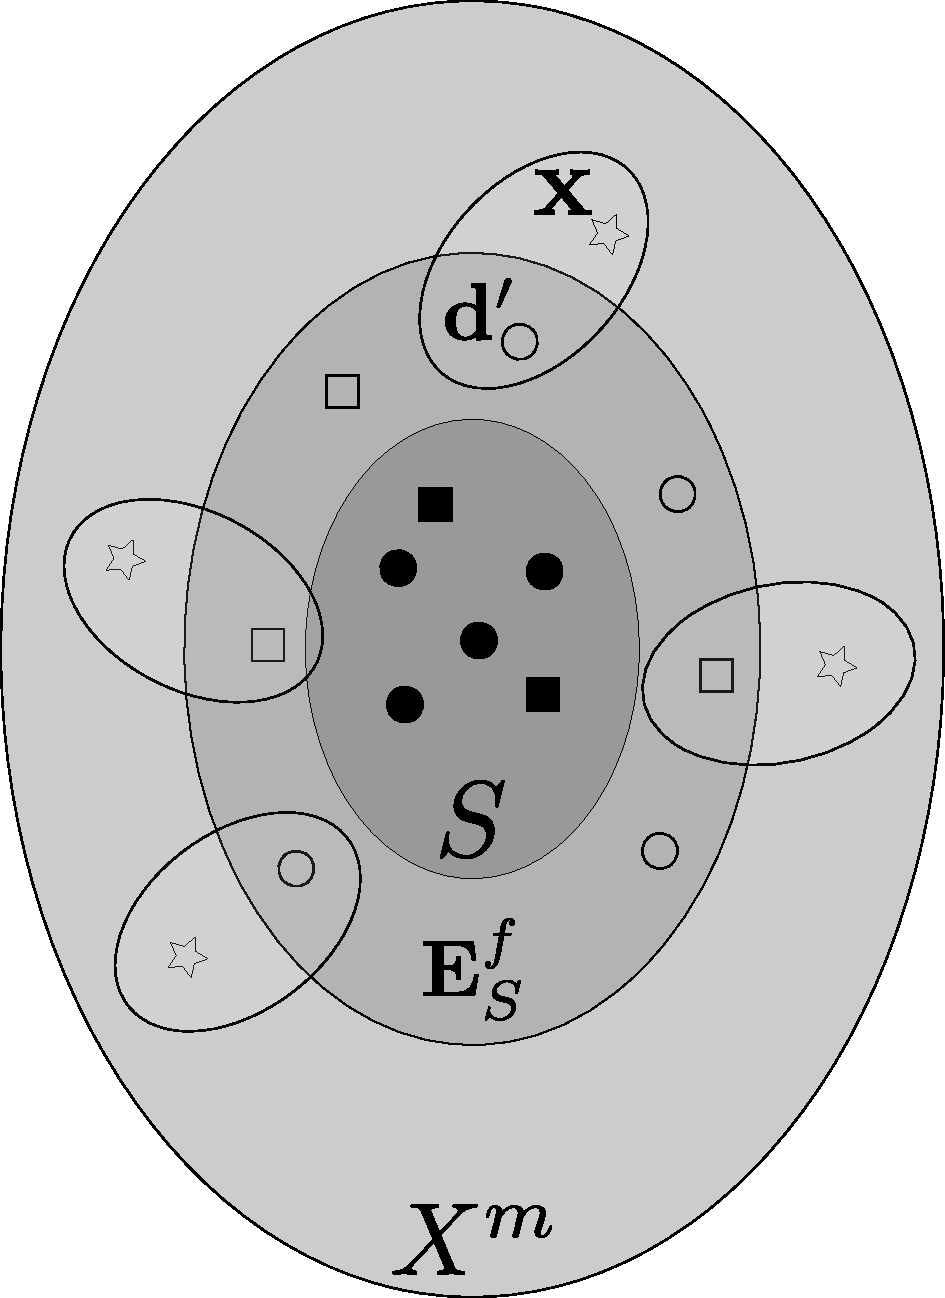
\includegraphics[scale=0.20]{figures/extended_classifier.pdf}
\end{center}
  \caption{Classification process of an extended analogical learner.
  $\hat{f}(\mathbf{x}) = \albl{\mathbf{d}'}$.}
\label{FIG:extended_classifier}
\end{figure}
Let us note that topologically speaking, Figure \ref{FIG:extended_classifier}
is not representative of a real case: even if we always have $S \subseteq \esf
\subseteq X^m$, this does not mean that these sets are embedded into one
another as shown in the drawing. Actually, if the underlying probability
distribution of $X^m$ is uniform, the elements of $S$ (and thus of $\esf$) are
scattered over the whole universe.

\begin{testexample}
Going back (for the last time!) to Figure \ref{FIG:ae_example}, our
new functional view allows us to consider the following steps:
\begin{enumerate}
  \item First extend $S = \Set{\mathbf{a}, \mathbf{b}, \mathbf{d}, \mathbf{e}}$
    to $\esf = \Set{\mathbf{a}, \mathbf{b}, \mathbf{c}, \mathbf{d},
    \mathbf{e}}$ with $\hat{f}(\mathbf{c}) = \albl{\mathbf{c}} = 1$ and
    $\hat{f}(\mathbf{f}) = \albl{\mathbf{f}} = 1$.
  \item Then, to classify $\mathbf{g}$, we simply look to its nearest neighbors
    in $\esf$, which are $\mathbf{c}$ and $\mathbf{e}$. The aggregation of
    their analogical labels leads to
    $\hat{f}(\mathbf{g}) = 1$. The nearest neighbors of $\mathbf{h}$ are
    $\mathbf{d}$ and $\mathbf{f}$, which also leads to $\hat{f}(\mathbf{h}) =
    1$.
\end{enumerate}
\end{testexample}

As far as we know, this is the first time a functional definition of
analogy-based classifiers is given. This definition clearly fits with the known
algorithms but obviously, some implementation details cannot be exactly caught
up by such a high level description. It is indeed possible to find a few edge
cases where this functional definition may not output the same result as
algorithm \ref{ALGO:extended_classifier}: this is the case for example when the
nearest analogical neighbor (nan) of $\mathbf{x}$ is not unique. It is also the
case with the Boolean proportion when the closest vertex $\mathbf{d}'$ does not
belong to $\mathbb{B}^m$.  However, as we will see later, these cases are not
likely to occur and the two approaches (that of Algorithm
\ref{ALGO:extended_classifier} and that of Definition
\ref{DEF:extended_classifier}) produce very similar results, thus empirically
validating this functional definition.

Since we now have a clear functional definition of analogical classifiers, we
are in position to examine some general theoretical properties of analogical
learners. This is the purpose of the next section.
\section{Theoretical properties of analogical classifiers}
\label{SEC:theoretical_properties_of_analogical_classifiers}

The functional definition of analogical learners opens the door to the study of
various theoretical properties of analogical classifiers, which had only been
described algorithmically so far. Just like for the $k$-NN literature,
theoretical results are easier to derive when $k = 1$. We will therefore mostly
focus on the properties of the 1-NAN classifier.
\subsection{Study of convergence}

Let us consider the case where $X^m=\mathbb{R}^m$, and let $\delta$ be any
distance function defined from a norm. Simply because $S \subseteq \esf$ for
any $S$, the
following inequality holds for any $\mathbf{x} \in X^m$ :
$$\delta(\mathbf{x}, \nan(\mathbf{x},S)) \leq \delta(\mathbf{x},
\nn(\mathbf{x},S)).$$


Now, let us consider  $\mathbf{x}^{(i)}$ an i.i.d. sequence of random variables
in $\mathbb{R}^m$, where $\mathbb{R}^m$ is equipped with a probability measure
denoted $P$. The training set will be denoted
$S_n=\Set{\left(\mathbf{x}^{(i)},f(\mathbf{x}^{(i)}) \right), ~ i
\in [1, n]}$. As $S_n$ is random, then $\nan(\mathbf{x},S_n)$ can also be
considered as a random element of $X^m$.  We then are exactly in the same
context as the work of Cover \& Hart who studied the 1-NN algorithm
(\cite{CovHarTIT67}), and we obtain a similar result:
\begin{property}
  \label{PROPER:convergence_nan}
  For any $\mathbf{x}$, its nan $\nanemph(\mathbf{x}, S_n)$ converges almost
  surely towards $\mathbf{x}$ as $n$ tends to infinity:
  $$P\left(\lim_{n \to \infty} \nanemph(\mathbf{x}, S_n) = \mathbf{x}\right) =
  1.$$
\end{property}
\begin{proof}
  The proof can be easily derived from the results of Cover \& Hart in
  \cite{CovHarTIT67}. Indeed, they have already showed that the nearest neighbor of
  $\mathbf{x}$ converges almost surely towards $\mathbf{x}$ as $n$ tends to
  infinity:
  $$P\left(\lim_{n \to \infty} \nn(\mathbf{x}, S_n) = \mathbf{x}\right) =
  1.$$
  To prove this result, they simply start from the fact that
  $\delta(\mathbf{x}, \nn(\mathbf{x}, S_n))$ converges in probability towards
  $0$:
  $$\forall \epsilon > 0,~~P\Big(\delta(\mathbf{x}, \nn(\mathbf{x}, S_n)) >
  \epsilon\Big) = 0.$$
  Using the previous fact that $\delta(\mathbf{x}, \nan(\mathbf{x},S_n)) \leq
  \delta(\mathbf{x}, \nn(\mathbf{x},S_n))$, the convergence in probability of
  $\delta(\mathbf{x}, \nan(\mathbf{x},S_n))$ towards $0$ is immediate. Then, it
  naturally follows that $\nan(\mathbf{x}, S_n)$ converges almost surely
  towards $\mathbf{x}$, following the same steps as Cover \& Hart.
\end{proof}

Let us note the following points:
\begin{enumerate}
\item The result of Cover and Hart was actually proved in a less restrictive
  setting than ours. They have proven their result for any separable metric
    space, without any additional structure. Unfortunately, we are not able to
    follow these lines here, because there is no known way to define an
    analogical dissimilarity on a metric space, without the help of any other
    structure or operator (see \cite{MicBayDelJAIR08} for a detailed discussion
    on this issue).
  \item Cover \& Hart proved that when $n$ tends to infinity, the probability
    of error of the 1-NN classifier is less than twice that of the Bayes
    probability of error, and therefore less than twice the probability of error of
    any other classifier. We have not been able to prove such a strong result
    for the $1$-\NAN~classifier, but its probability of error will be thoroughly
    investigated in Subsection \ref{SEC:accuracy_analysis}.
  \item We have to be careful about the interpretation of Property
    \ref{PROPER:convergence_nan} in terms of machine learning. Indeed, another
    key property is proved in \cite{CovHarTIT67}: for an integrable
    function $f$  over $\mathbb{R}^m$ with regards to the probability measure $P$, the
    expectation of $f(\nn(\mathbf{x},S_n))- f(\mathbf{x})$ converges to 0 when
    $n$ tends to infinity.  This means that asymptotically, the nearest
    neighbour of $\mathbf{x}$ has the same properties as $\mathbf{x}$, and
    particularly: \textbf{they have the same label}, which is a very powerful
    property when we are dealing with a classification task. Sadly, such a
    property has not been proven for $\nan(\mathbf{x}, S_n)$.
\item Finally, it is clear that when $n$ goes to infinity, the behavior of an
  analogical classifier tends to that of a nearest neighbours classifier.
    Indeed, when $S_n$ is very big, the nearest analogical neighbour of an
    element $\mathbf{x}$ simply is its nearest neighbour, in most cases.
    Moreover, when the nan and the nn are too close, paying the price of the
    noise related to the nan may not be worth it. This supports the common
    acknowledgement that analogical reasoning is mostly useful when very few
    data are available.  In this latter case, extending a small training set with
    its analogical extension may be particularly beneficial, as we will see in
    Chapter \ref{CHAP:analogy_preserving_functions}.

\end{enumerate}
To conclude this discussion, even if the convergence result is interesting in
itself, it does not say a lot in terms of machine learning. A much more
interesting and powerful theoretical result of analogical classifiers will be
proven in Chapter \ref{CHAP:analogy_preserving_functions}. Let us now focus on
their VC-dimension.

\subsection{Vapnik Chervonenkis (VC) dimension of analogical classifiers}
\label{SEC:VCdim}
The notion of VC-dimension was originally defined by Vapnik and Chervonenkis
\cite{Vap98}, and introduced into learnability theory by Blumer et al.
\cite{BluEhrHauWarACM89}. Roughly speaking, the VC-dimension (denoted VC) of a class of
learners is a numerical measure of their discrimination power. One of the main
results about the VC-dimension is that it allows to bound the true risk $R$ of
a learner. With probability $1 - \eta$, and under some theoretical conditions
that we omit here, we have:

$$R \leq R_{\text{emp}} + \sqrt{\frac{1}{n} \cdot \left[\text{VC}(\log(2n /
\text{VC}) + 1) - \log(\eta/4)\right]},$$
where $R_\text{emp}$ is the probability of error on a training set $S_n$, and
VC is the VC-dimension of the learner. In our setting,
\begin{itemize}
  \item $R \eqdef P\left(\hat{f}(\mathbf{x}) \neq f(\mathbf{x}) \given[\big]
    \mathbf{x} \in X^m\right)$, and
  \item $R_\text{emp} \eqdef P\left(\hat{f}(\mathbf{x}) \neq f(\mathbf{x})
    \given[\big] \mathbf{x} \in S_n\right)$.
\end{itemize}

This theoretical upper bound on the true risk $R$ is what makes the
VC-dimension of a class of learners an essential element of their theoretical
study. The VC-dimension is defined as follows:

\begin{definition}[VC-dimension]
  \label{DEF:VCdim}
  We consider a class of learners $\mathcal{C}$ and a set $S_n$ of $n$ labeled
  elements in $X^m$. There are exactly $2^n$ ways to label each of the $n$
  elements. If for any labeling, there exists a learner in $\mathcal{C}$ that
  correctly labels all the elements in $S_n$, we say that $\mathcal{C}$
  \textbf{shatters} $S_n$.
  The \textbf{VC-dimension} of $\mathcal{C}$ is the biggest $n$ such that there exists a
  set of $n$ points $S_n$ that can be shattered by $\mathcal{C}$.  When there
  exists a set $S_n$ that can be shattered for any size $n$, we say that the
  VC-dimension is infinite.
\end{definition}


Let's first consider the class of nearest neighbors classifiers:
$\mathcal{C}_{\text{NN}}=\{ k\text{-NN classifiers}, k \in \mathbb{N}^*\}$. It
is clear that the VC-dimension of $\mathcal{C}_{\text{NN}}$ is infinite: taking
$k = 1$, any training set of any size can be perfectly labeled by 1-NN,
because every element is its own nearest neighbor. Actually, we can easily show
the same result for the analogical learners.

\begin{proposition}
  \label{PROPOS:VCdim}
  The class $\mathcal{AC}_k$ of analogical learners has infinite VC-dimension.
\end{proposition}
\begin{proof}
  Considering Definition \ref{DEF:extended_classifier} on page
  \pageref{DEF:extended_classifier} with $k = 1$, we see
  that the predicted label of any element $\mathbf{x}$ is that of its nan. For
  any element $\mathbf{x}$ in $S_n$, $\mathbf{x}$ is its own nan (just like
  $\mathbf{x}$ is its own nearest neighbor). Hence, any training set $S_n$ of
  size $n$ is correctly labeled by 1-NAN, and thus can be shattered by
  $\mathcal{AC}_k$. Therefore, the VC-dimension of $\mathcal{AC}_k$ is infinite.
\end{proof}

Clearly, the upper bound of the true risk is a decreasing function in $n$, and an increasing
function in the VC dimension of the learner. As such, we usually want the
VC-dimension of our classifiers to be small. However, we have previously seen
that the nearest neighbors classifiers, despite their infinite
VC-dimension, enjoy many interesting theoretical properties, and their
practical efficiency is well-acknowledged. In fact, the upper bound on the true
risk does not even hold for classes of learner whose VC-dimension is infinite
\cite{Bur98}. We then need to keep in mind that even though the analogical
learners have an infinite VC-dimension, which is an interesting result in its
own right, this does not necessarily prevent them from being useful
classifiers.

\subsection{Accuracy analysis}
\label{SEC:accuracy_analysis}

In this section, we study the accuracy of an analogical classifier, and more
particularly that of the $\NAN$ classifier. As explained in Section
\ref{SEC:functional_definition}, for a given $\mathbf{x} \in X^m$ and a
training set $S \subset X^m$, the prediction $\hat{f}(\mathbf{x})$ is set as:
$$
\hat{f}(\mathbf{x}) ~ \eqdef ~ \albl{\nan(\mathbf{x}, S)} ~ \eqdef ~ \albl{\nn(\mathbf{x}, \esf)}.
$$

We now equip the set $X^m$ with a probability distribution denoted $P$.  The
accuracy of the $\NAN_S$ classifier\footnote{The $S$ subscript is here to
specify that the training set of the $\NAN$ algorithm is $S$. The same notation
is used for the \textit{nearest neighbour} algorithm: $\NN_\Sigma$ is the $\NN$
algorithm trained on the set $\Sigma$.} over all the elements of $X^m$ is
defined as:
$$\acc(\NAN_S, X^m)\eqdef P\left(\hat{f}(\mathbf{x})=f(\mathbf{x}) \given[\big]
\mathbf{x} \in X^m\right).$$
Our main result is given by Proposition \ref{PROPOS:accuracy_nan}:
\begin{proposition}
  \label{PROPOS:accuracy_nan}
  The accuracy of $\NAN_S$ over $X^m$ can be seen as the weighted sum of the
  accuracy of $\NN$ over $A$ and $B$, using a different training set each time
  (respectively $S$ and $\esfs$):
  \begin{align*}
    \acc(\NAN_S, X^m) = ~&\acc(\NN_S, A) \cdot \alpha ~ + \\
                        &\acc(\NN_{\esfs}, B) \cdot (1 - \alpha),
  \end{align*}
  where:
  \begin{itemize}
  \item $A \eqdef \set{\mathbf{x} \in X^m | \nan(\mathbf{x}, S) \in S}$: the
    elements that have their nan in $S$.
  \item $B \eqdef \set{\mathbf{x} \in X^m | \nan(\mathbf{x}, S) \in \esfs}$: the
    elements that have their nan in $\esfs$.
  \item $\alpha \eqdef P(\mathbf{x} \in A)$ and $1 - \alpha = P(\mathbf{x} \in
    B)$. 
  \end{itemize}
  Naturally, $A \cup B = X^m$ and $A \cap B = \varnothing$.
\end{proposition}
\begin{proof}
By observing that for any $\mathbf{x}$, its $\nan$ either belongs to $S$ or to
$\esfs$, the accuracy $\acc(\NAN_S, X^m)$ can be split into two distinct parts as follows:

\begin{align*}
  &\acc(\NAN_S, X^m) \eqdef P\left(\hat{f}(\mathbf{x})=f(\mathbf{x}) \given[\big] \mathbf{x} \in
  X^m\right) = P\left(\albl{\nan(\mathbf{x}, S)} = f(\mathbf{x})\right)\\
  =~&P\left([\albl{\nan(\mathbf{x}, S)} = f(\mathbf{x}) ]\wedge
  [\nan(\mathbf{x}, S) \in S ] \right)~ +
  P\left([\albl{\nan(\mathbf{x}, S)} = f(\mathbf{x})] \wedge [\nan(\mathbf{x},
  S) \in \esfs]\right)\\
  =~&P\left([\albl{\nn(\mathbf{x}, \esf)} = f(\mathbf{x})] \wedge
  [\nn(\mathbf{x}, \esf) \in S ]\right)~ +
  P\left([\albl{\nn(\mathbf{x}, \esf)} = f(\mathbf{x})] \wedge
  [\nn(\mathbf{x}, \esf) \in \esfs]\right) \\
  =~&P\left([\albl{\nn(\mathbf{x}, \esf)} = f(\mathbf{x})] \given[\big]
  [\nn(\mathbf{x}, \esf) \in S ]\right) \times
  P\left([\nn(\mathbf{x}, \esf) \in S]\right) ~+ \\
  &P\left([\albl{\nn(\mathbf{x}, \esf)} = f(\mathbf{x})] \given[\big]
  [\nn(\mathbf{x}, \esf) \in \esfs]\right) \times
  P\left([ \nn(\mathbf{x}, \esf) \in \esfs]\right)
\end{align*}

Let us denote  $\alpha \eqdef P\left(\nn(\mathbf{x}, \esf) \in S\right)$.
Obviously, we also have $\alpha \eqdef P\left(\nan(\mathbf{x}, S) \in
S\right)$.  The above formula becomes:
\begin{align*}
  &\acc(\NAN_S, X^m) = \\&P\left([\albl{\nn(\mathbf{x}, \esf)} = f(\mathbf{x})]
  \given[\big] [\nn(\mathbf{x}, \esf) \in S] \right) * \alpha ~+ \\
  &P\left([\albl{\nn(\mathbf{x}, \esf)} = f(\mathbf{x})] \given[\big]
  [\nn(\mathbf{x}, \esf) \in \esfs]\right) * (1 - \alpha).
\end{align*}

Let us focus on the first term, temporarily discarding the factor $\alpha$:
$$P\left([\albl{\nn(\mathbf{x}, \esf)} = f(\mathbf{x})] \given[\big]
[\nn(\mathbf{x}, \esf) \in S] \right).$$

It is easy to see that the event $[\nn(\mathbf{x}, \esf) \in S]$ is equivalent
to the event $[\nn(\mathbf{x}, \esf) = \nn(\mathbf{x}, S)]$. As a result, we
can transform the first term to get a better grasp of its meaning:
\begin{align*}
  &P\left([\albl{\nn(\mathbf{x}, \esf)} = f(\mathbf{x})] \given[\big]
  [\nn(\mathbf{x}, \esf) \in S] \right)\\
  =~ &P\left([\albl{\nn(\mathbf{x},\esf)} = f(\mathbf{x})] \given[\big]
  [\nn(\mathbf{x}, \esf) = \nn(\mathbf{x}, S)]\right)\\
  =~ &P\left([\albl{\nn(\mathbf{x}, S)} = f(\mathbf{x})] \given[\big]
  [\nn(\mathbf{x}, \esf) \in S]\right).
\end{align*}

In this form, the first term is just the accuracy of the $\NN_S$ algorithm over
the elements that have their nearest analogical neighbour in $S$.
As for the second term, the same process can be applied by observing that the
event $[\nn(\mathbf{x}, \esf) \in\esfs]$ is equivalent to the event
$[\nn(\mathbf{x}, \esf) = \nn(\mathbf{x}, \esfs)]$. This leads to
\begin{align*}
  &P\left([\albl{\nn(\mathbf{x}, \esf)} = f(\mathbf{x})] \given[\big]
  [\nn(\mathbf{x}, \esf) \in \esfs]\right)\\
  =~ &P\left([\albl{\nn(\mathbf{x}, \esfs)} = f(\mathbf{x})] \given[\big]
  [\nn(\mathbf{x}, \esf) \in \esfs]\right).
\end{align*}

This second term is then the accuracy of the $\NN_{\esfs}$ algorithm over the
elements that have their nearest analogical neighbour in $\esfs$.

In the light of these interpretations, we can directly rewrite the accuracy
formula in the concise form given in Proposition \ref{PROPOS:accuracy_nan}.
\end{proof}

The value $\acc(\NN_S, A)$ is the accuracy of $\NN_S$ over all the elements in
$A$. A theoretical study of this accuracy has been done in \cite{LanIbaIJCAI93}
when the size of $A$ is known.  Regarding $\acc(\NN_{\esfs}, B)$, this is the
accuracy of $1$-$\NN$ when the training set is
noisy, and has been studied in \cite{OkaYugIJCAI97}. This last formula leads
to the consistent facts:
\begin{enumerate}
\item The smaller $\esfs$ (i.e. analogical reasoning does not
  bring much more labels), the closer $\alpha$ is to $1$, the closer $A$ is to
  $X^m$ and the more the accuracy of $\NAN_S$ tends towards the accuracy of
  $\NN_S$ over $X^m$.
\item In return, if $\esf$ is much bigger than $S$, $\alpha$ is then small, $B$
  is close to $X^m$ and the accuracy of $\NAN_S$ greatly depends on the quality
  of $\esf$:  \end{enumerate}

\begin{definition}[Quality of the analogical extension $\omegasf$]
  \label{DEF:omega}
  Given a training set $S\subset X^m$ and a ground truth function $f$, the
  \textbf{quality} of the analogical extension $\esf$ is defined as:
  $$
  \omegasf \eqdef P\left(\albl{\mathbf{x}} = f(\mathbf{x}) \given[\big]
  \mathbf{x} \in \esfs\right).$$
  Note that the value $1 - \omegasf$ corresponds to the class noise of $\esfs$.
\end{definition}

This closes our contributions to the theoretical properties of analogical
classifiers. In the next section, we will empirically investigate and illustrate the
soundness of our results.

\section{Experiments and empirical validation}
\label{SEC:experiments_and_empirical_validation}
In order to get an empirical validation of our formulas, we have developed a
set of experiments that we now describe.

\subsection{Evaluation protocol}

Working with Boolean vectors, we have computed the accuracies of the 1-\NAN~and
1-$\NN$~ algorithms over $X=\mathbb{B}^m$ for $m = 8$. Other values of $m$ have
been investigated, leading to very similar results.  The ground truth label of
the elements of $X^m$ is defined by different Boolean functions $f$:
\begin{itemize}
\item $f_1(\mathbf{x})=x_i$ for some $i$. These functions are called
  projections, or dictators.  They lead to perfectly linearly separable
    problems, i.e. there exists an hyperplane that can perfectly discriminate
    both classes. As such, they are expected to be fairly easy to learn.
  \item $f_2(\mathbf{x})= \bigoplus_{i = 1}^k  x_i$ for some $k \in[1, m]$, where $\oplus$
    is the XOR operator (which is associative). These functions
    lead to highly non-linearly-separable problems: remember the example of
    Figure \ref{FIG:classification_problem} on page
    \pageref{FIG:classification_problem}, who was an instance of a XOR problem.
    XOR problems are traditionally difficult to learn.
  \item $f_3(\mathbf{x})= \bigwedge_{i = 1}^k  x_i$ for some $k \in [1, m]$.
  \item $f_4(\mathbf{x})= \bigvee_{i = 1}^k  x_i$ for some $k\in [1, m]$.
  \item $f_5(\mathbf{x}) = \left[\sum_{i = 1}^m x_i \geq k\right]$ for some $k
    \in [1, m]$, where the function $[\text{cond}]$ is equal to $1$ if cond is
    verified and $0$ else. Simply put, $f(\mathbf{x}) = 1$ iff at least $k$
    components are equal to $1$.
  \item $f_6(\mathbf{x}) = \left[\sum_{i = 1}^m x_i = k\right]$ for some $k
    \in [1, m]$. Simply put, $f(\mathbf{x}) = 1$ iff exactly $k$ components
    are equal to $1$.
\end{itemize}


Regarding the size of the training set, to be sure to fit with the size of the
universe, we have investigated various sizes between $3$ and $100$. When
dealing with a training set of size $100$, the cubic complexity of the
analogical classifier leads to explore a set of approximately $100^3$ elements:
as a consequence, we limit our investigation to a maximum of 100 elements in
the training set in order to get a realistic execution time.

All the accuracy (and other metrics) computations are averaged over a set of
100 experiments. We have made sure that the class distributions of the training
sets are as close as possible to that of the whole universe $X^m$.  Note that
our implementation of the $\NAN$ algorithm is not that of algorithm
\ref{ALGO:extended_classifier}, but is instead that of the functional
definition of the analogical classifier as described in Definition
\ref{DEF:extended_classifier}: we first construct the analogical extension set
of $S$, and then proceed to a nearest neighbour strategy over this noisy
extended training set. We have estimated probabilities by frequencies, thus
implicitly assuming a uniform distribution on $X^m$.

For each experiment, we have computed the following measures to empirically
investigate the behaviour of the analogical classifier, and assess our
theoretical results:
\begin{itemize}
  \item The empirical accuracy of the 1NAN classifier, defined\footnote{We
    notice here that $\mathbf{x}$ is only required to belong to $X^m \setminus
    S$ and not to $X^m$, because classifying elements in $S$ is pointless.}
    as\\
    $\acc(\NAN_S) \eqdef P\left(\hat{f}(\mathbf{x}) = f(\mathbf{x})
    \given[\big] \mathbf{x} \in X^m \setminus S \right)$.
  \item The empirical accuracy of the 1NN classifier, whose definition is of
    course the same but this time $\hat{f}$ is the output of the 1NN
    classifier.
  \item The \textbf{theoretical} accuracy of 1NAN, as defined in Proposition
    \ref{PROPOS:accuracy_nan}. The probability $\alpha \eqdef P(\mathbf{x} \in
    A$) has been estimated by the frequency $\frac{\mid A \mid}{\mid X^m
    \mid}$. Both sets $A$ and $B$ are easy to determine.
  \item The quality of $\esf$, measured by $\omegasf$ as previously defined in
    Definition  \ref{DEF:omega}. $\omegasf$ has been estimated by the
    frequency $\frac{\big| \Set{\mathbf{x} \in \esfs | \albl{\mathbf{x}} =
    f(\mathbf{x}}\big|}{\big| \esfs \big|}$.
  \item Finally, the quantity $\gamma_S^f \eqdef P(\mathbf{x} \in \esf)$,
    estimated by $\frac{\mid \esf\mid}{\mid X^m \mid}$: the size of the
    analogical extension with respect to that of the whole universe.
\end{itemize}

It is fairly easy to see that both functions $f_1$ and $f_2$ split the universe $X^m$ into
two disjoint sets of size $2^{m - 1}$: those for which $f(\mathbf{x})$ is
equal to $1$, and those with labels equal to $0$. We say that the datasets are
balanced. However, the other functions may lead to very unbalanced datasets. An
extreme case is for example $f_3$ with $k = m$, which leads to $f_3(\mathbf{x})
= x_1 \wedge x_2 \wedge \dots \wedge x_m$. The only element whose label is $1$
is the vector $\mathbf{x} = (1, 1, \dots, 1)$. For these very unbalanced
datasets, the accuracy of a classifier is not a relevant measure: predicting
$0$ all the time would lead to an accuracy of almost $1$, but would
systematically assign the wrong label to   $(1, 1, \dots 1)$. Therefore, as
accuracy is our main concern here, we will focus on functions for which
datasets are as balanced as possible.

In addition to these Boolean functions, we have also run the $\NAN$ algorithm
over the Monk datasets over the UCI
repository\footnote{\url{https://archive.ics.uci.edu/ml/datasets/MONK's+Problems}}.
They are datasets of 432 binarized elements, among which exactly 169 of them
have been used for training.

\subsection{Comments and discussion}

Our experiments are summed-up by Figure \ref{FIG:nan_vs_nn} on page
\pageref{FIG:nan_vs_nn}. As they are the result of multiple averaged
experiments, the measures $\omegasf$ and $\gamma_S^f$ are here denoted $\omega$
and $\gamma$. Paying careful attention to these plots will allow us to draw
interesting conclusions about the behaviour of the 1-NAN algorithm.

\begin{figure}[!h]
\centering
  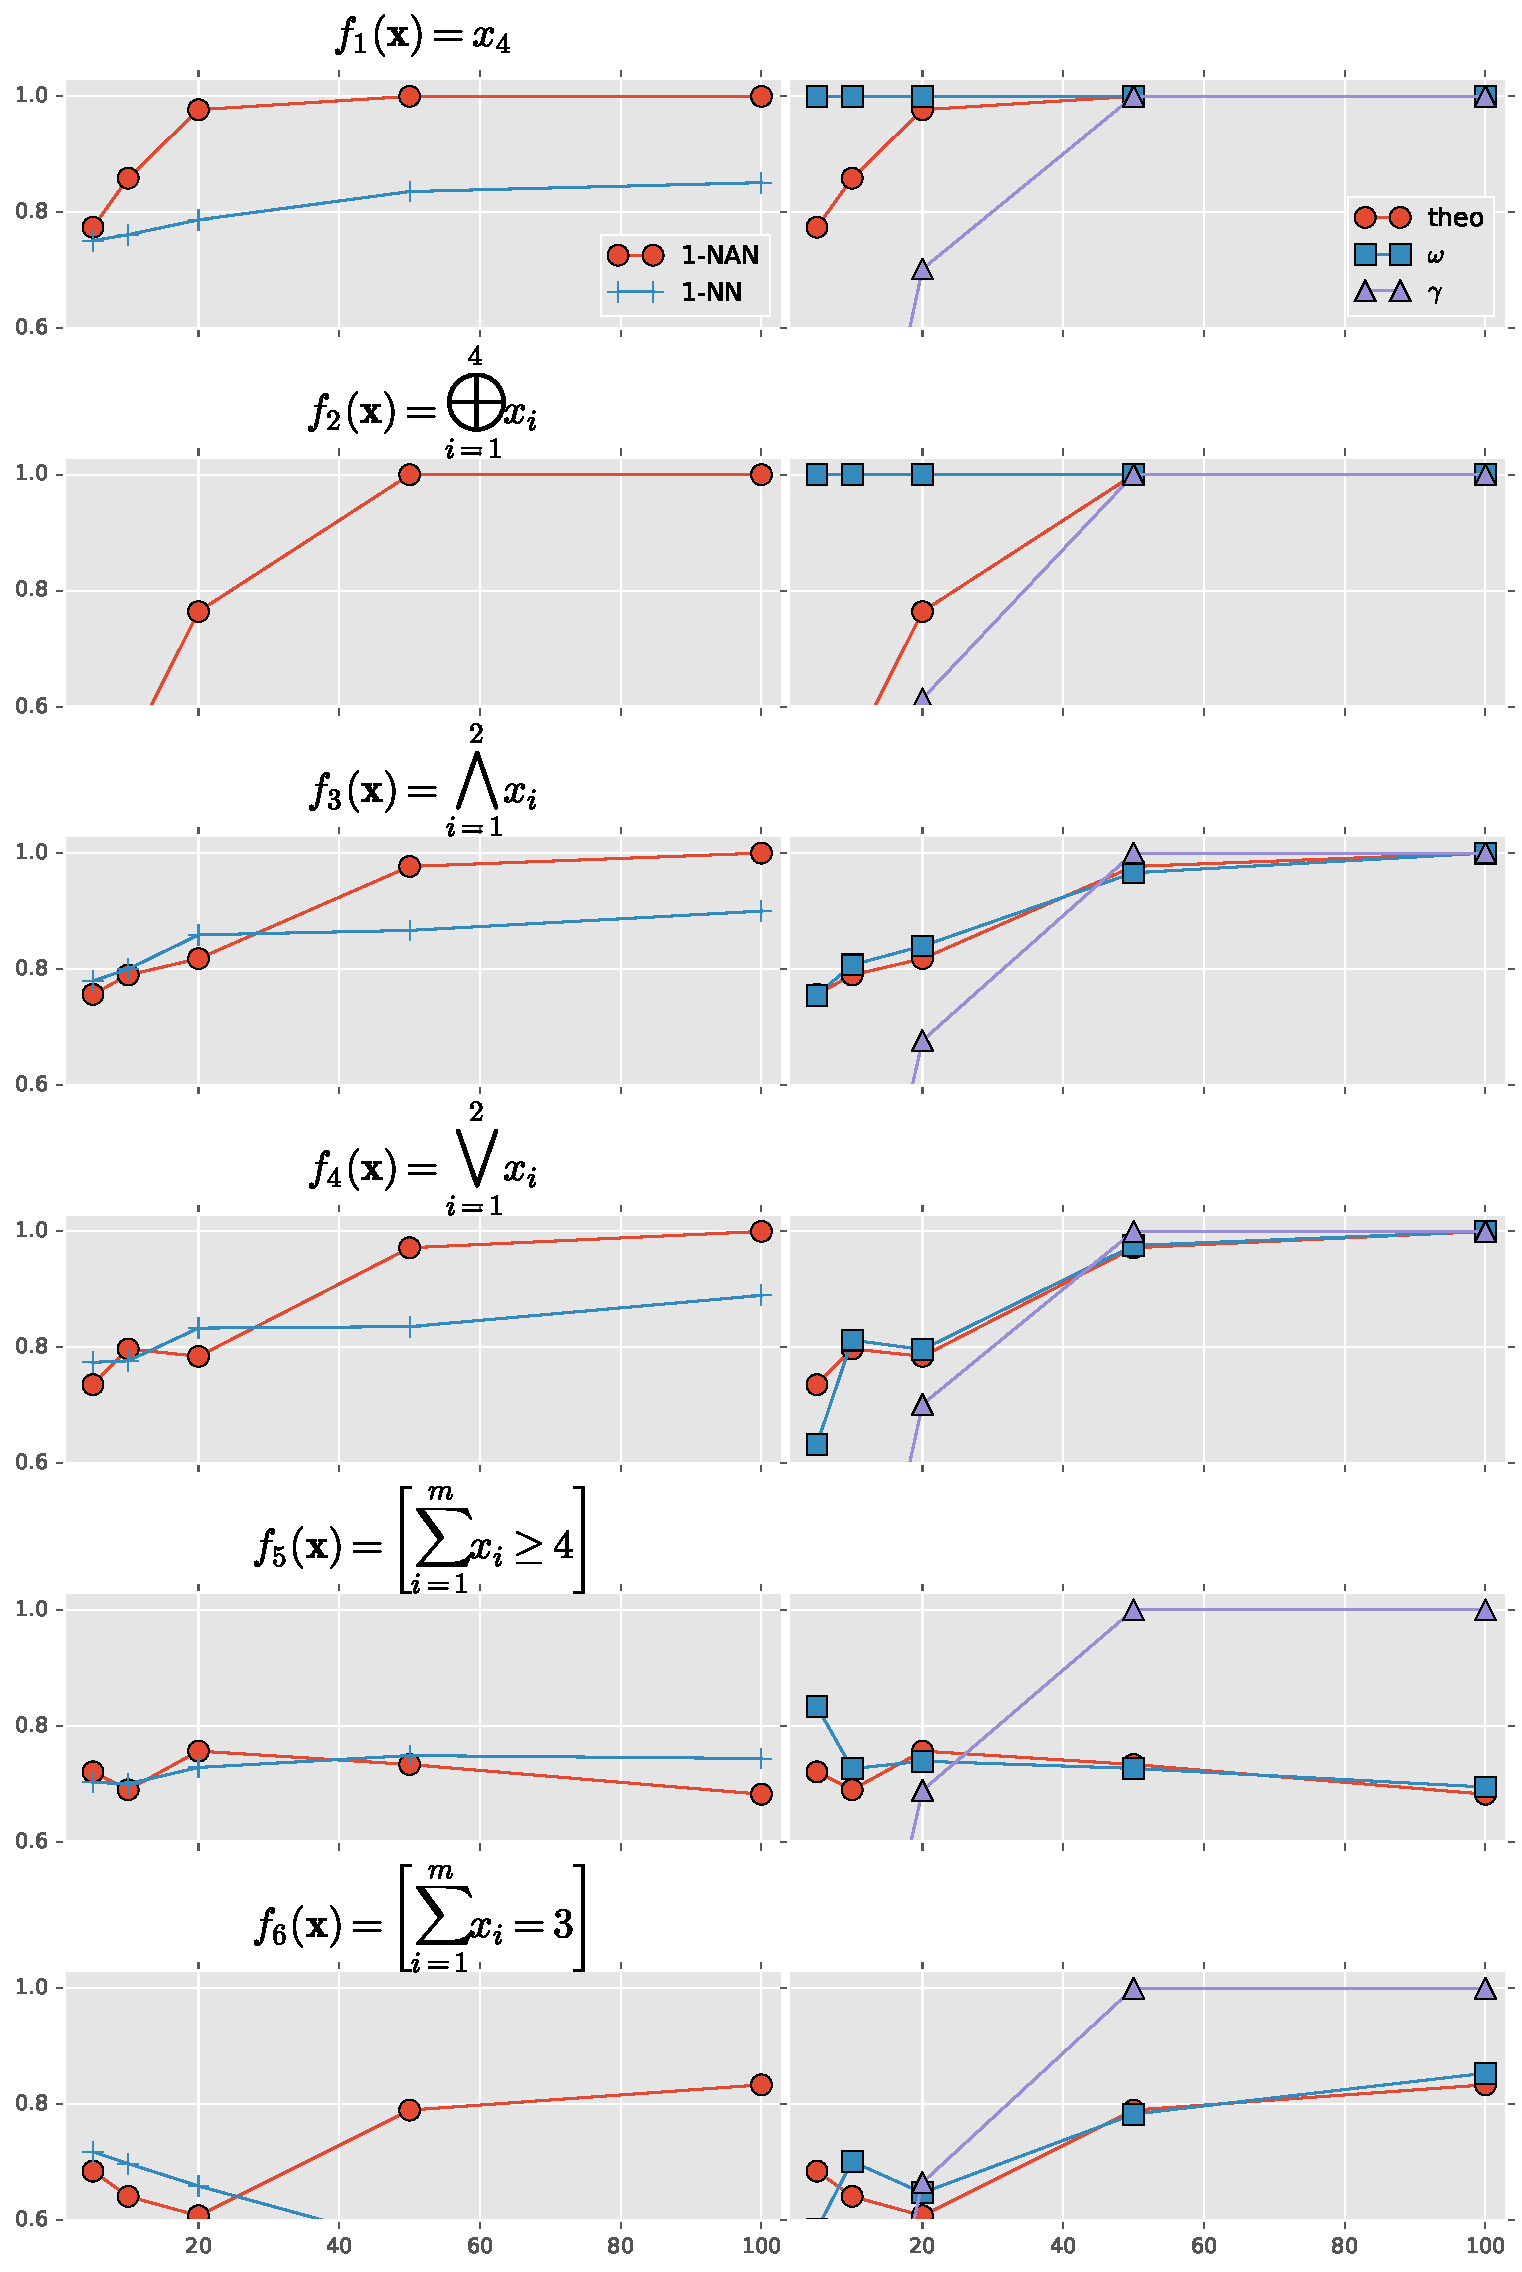
\includegraphics[scale=.50]{figures/nan_vs_nn_SUMMARY_dim8_nexp15.pdf}
  \caption{Accuracies (left) of the 1-NAN and 1-NN algorithms over different
  Boolean functions ($m = 8$) and training set sizes, with corresponding values
  of $\omega$, $\gamma$, and theoretical accuracy (right). The $x$ axis
  corresponds to the size of the training set.}
\label{FIG:nan_vs_nn}
\end{figure}

First, the theoretical accuracy seems to fit perfectly with the empirical
accuracy of the $\NAN$ algorithm, thus validating our theoretical study that
led to proposition \ref{PROPOS:accuracy_nan}. Actually, the maximal difference
we observed between the theoretical accuracy and its actual value is of about
$10^{-10}$.

An interesting observation is that the value of $\omega$ seems to always
converge to that of the theoretical accuracy (and therefore to the actual
accuracy) of $\NAN$. This can be easily explained by paying attention to the
value of $\gamma$, the proportion of elements of $X^m$ that belong to $\esf$.
We see that in any setting, $\gamma$ converges to 1 as $\mid S \mid$ grows.
This means that when $\mid S \mid$ is big enough (but not necessarily
\textit{that} big with respect to $X^m$), the analogical extension of $S$
covers the whole universe $X^m$ (obviously, the bigger the dimension $m$, the
slower the convergence occurs): every element $\mathbf{x}$ is then its own
nearest analogical neighbour and $\hat{f}(\mathbf{x}) = \albl{\mathbf{x}}$. It
is therefore straightforward to see that in this case,
$$
  \omega \eqdef P\left(\albl{\mathbf{x}} = f(\mathbf{x}) \given[\big]
  \mathbf{x} \in \esfs\right) = P\left(\hat{f}(\mathbf{x}) = f(\mathbf{x})
  \given[\big] \mathbf{x} \in \esfs\right)\\ = \acc(\NAN_S, \esfs).
$$
When $\gamma = 1$, the only elements $\mathbf{x}$ we want to classify belong to
$\esfs$ (otherwise they would be in $S$), so this last term exactly corresponds
to the accuracy of the classifier. Another way to see it is to observe that the
first term of the expression of Proposition (\ref{PROPOS:accuracy_nan})
$\acc(\NN_{S}, A) \cdot \alpha$ is zero
because $\alpha = 0$. Only the second term $\acc(\NN_{\esfs}, B) \cdot (1 -
\alpha)$ is of importance, and its value corresponds to $\omega$. As expected,
this observation allows us to state that estimating the value of $\omega$ is
paramount to have a precise idea of the accuracy of an analogical classifier.
%We will provide in the next subsection a method to accurately estimate this
%quantity $\omega$ with the only help of the training set $S$.

A striking result of the experiments is that for the two functions
$f_1(\mathbf{x}) = x_4$ and $f_2(\mathbf{x}) = x_1 \oplus \cdots \oplus x_4$,
the analogical labels are always correctly predicted: $\omega = 1$, i.e. there
is no class noise. However, the accuracy of 1-NAN is not necessarily equal to
$1$ especially for $f_2$ with small training set sizes. The reason is simple:
even if all the elements in $\esf$ are correctly classified, $\esf$ does not
cover the whole space ($\gamma < 1$) so the accuracy of 1-NAN still depends on
that of 1-NN. While the accuracy of 1-NN over $f_1$ is not too bad, the one
over $f_2$ is absolutely terrible and actually below $0.3$ (a random prediction
would have done better!). This is one of the distinguishing features of the XOR
functions: the nearest neighbor of an element is almost always in a different
class. So, sadly, the 1-NN algorithm can do nothing but wrong on these kind of
functions. In Chapter \ref{CHAP:analogy_preserving_functions}, we will prove a
strong result showing that both the projections (like $f_1$) and the XOR
functions (like $f_2$) \textbf{always} lead to perfectly sound extensions, for
any training set of any size.

Table \ref{TAB:monks} shows the same metrics for the Monk datasets and also
reports the results of the Analogical Proportion Classifier (\textit{APC}) from
\cite{MicBayDelJAIR08}, which corresponds to algorithm
\ref{ALGO:extended_classifier} with $k=100$.
\begin{table}
\centering
\begin{tabular}{ l  c  c c  c  c }
\toprule
& 1-NAN  & APC & 1-NN  &  $\omegasf$ & $\gamma_S^f$ \\
\midrule
Monk 1 & .961 & .98 & .787 &   .961    &   1 \\
Monk 2 & .998 & 1 & .738 &    .998    &   1 \\
Monk 3 & .963 & .96 & .829 &   .963    &   1 \\
\bottomrule
\end{tabular}
\caption{Accuracies of the 1-NAN, APC and 1-NN algorithms over the Monk
  datasets.}
  \label{TAB:monks}
\end{table}
We note that the functional $\NAN$ approach (almost) achieves the same results
as the somewhat more complex algorithm described in Section
\ref{SEC:extended_classifier}, and that here again the analogical extension set
covers the whole universe: this means that a conservative approach would have
been sufficient! Actually, this raises the following question: why would we
want to look for more than one analogical neighbour when every element of the
universe is already in $\esf$, and therefore \textit{analogically linked} to
those in $S$? Our experiments tend to show that this becomes superfluous,
provided that the training set is big enough.

%\subsection{Estimation of the prediction accuracy}
%
%We have seen in the previous subsection that the value $\omega$ is that of the actual
%accuracy of an analogical classifier when $S$ is big enough. This leads to the
%following question: how can we get a precise estimation of this value $\omega$
%? Answering this would allow us to have a very precise idea of the accuracy we
%can expect from our classifier.
%
%The method we propose for estimating $\omega$ only relies on the training set $S$
%and is very simple: it consists of applying the conservative algorithm to all
%the elements of $S$, and compute the fraction of these elements that have been
%correctly classified. A small yet important modification to the algorithm needs
%to be added: we only want to construct analogical proportions of the form $a :
%b :: c : x$ where $a$, $b$, $c$ and $x$ are all distinct elements. Indeed, the
%proportions $x : x :: x : x$ and $x' : x :: x' : x$ are always true, and the
%solution label related to these proportions would bias the final majority-vote
%procedure in a significant way towards the real label $\dot{x}$.
%
%We have applied this estimation protocol to all of the Boolean settings we have
%considered, and it has shown to be very accurate. Figure \ref{omegaplots}
%illustrates a few of these settings (already considered in Figure \ref{plots}).
%\begin{figure}
%  \caption{Values of $\omega$ and its estimation $\hat{\omega}$ for $f_1$, $f_2$ and $f_3$ in
%  $\mathbb{B}^{10}$.}
%\label{omegaplots}
%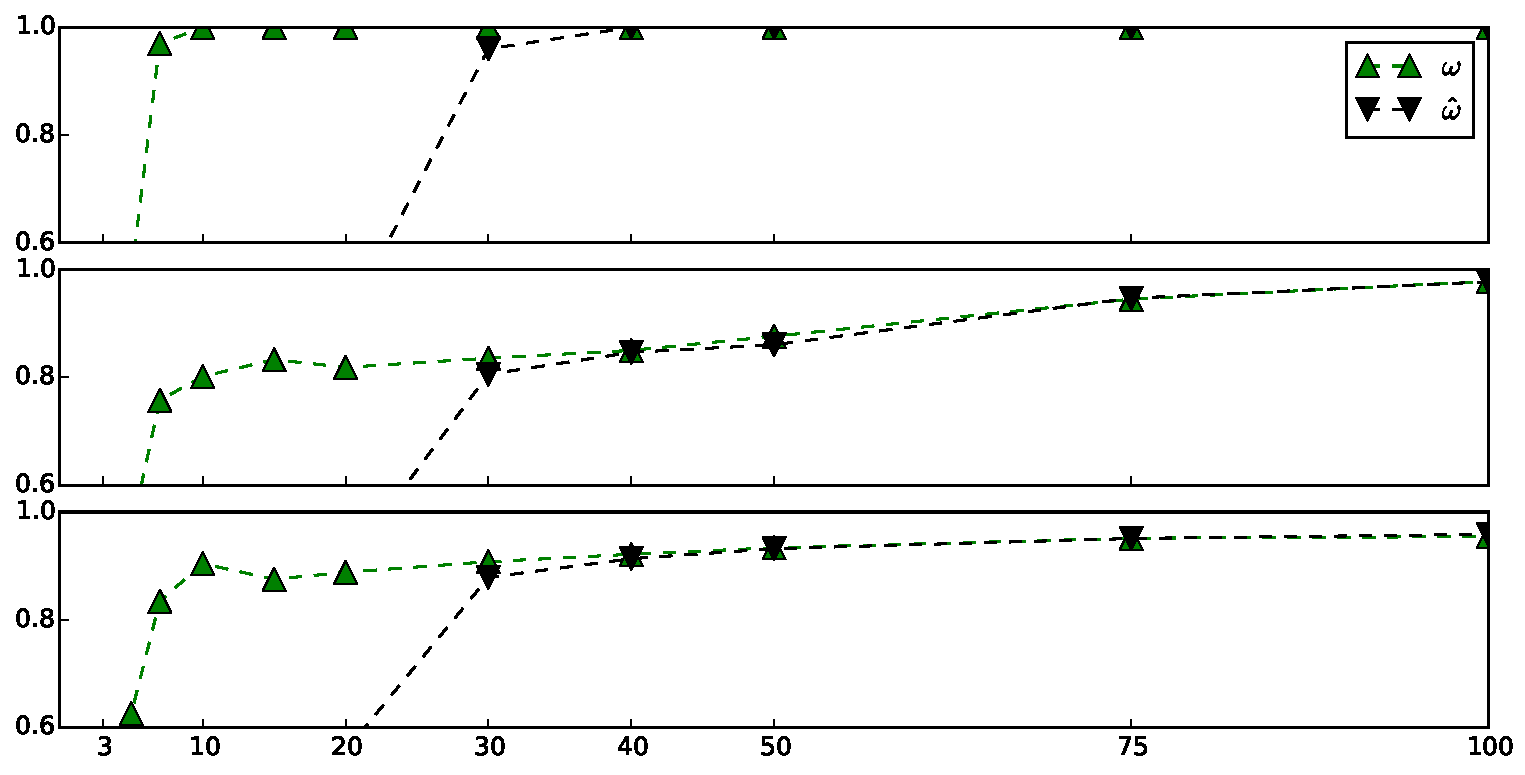
\includegraphics[width=\linewidth]{figures/ecai_estimation_omega.pdf}
%\end{figure}
%We can see that the estimation $\hat{\omega}$ converges to $\omega$ when $S$ is
%big enough. For small values of $S$, this estimation is indeed imprecise as it
%is difficult to find a lot a 3-tuples such that an analogical proportion holds
%for every element.

\section*{Conclusion}

In this Section, we have provided a functional and unifying definition of
analogical learners, which turned out to be closely related to the $k$-NN
classifiers. Starting from this definition, we were in a position to
prove an analytical convergence result, similar to that of the nearest neighbour
algorithm. Obviously, this is not enough to conclude regarding the predictive
ability of analogy-based classifiers. We have also shown that their
VC-dimension is infinite. It should not come as a surprise, as a very
particular case of analogical rule (when the analogical proportion is trivial)
is the $k$-NN rule.

This fact obviously has a consequence on the way we can
work to improve analogy-based classifier.  Indeed, learning by analogy is prone
to over-fitting and a relevant learning strategy should take this fact into
account.  Nevertheless, we have to keep in mind that the VC-dimension
alone is not a perfect marker of the quality of a machine learning algorithm,
especially when it comes to practical implementation.

In terms of accuracy in a Boolean setting, we have found a strong link between
the accuracy of the NAN algorithm and that of the NN algorithm. Our functional
definition tells us that we can consider the NAN algorithm as a NN strategy on an
extended and noisy training set: the analogical extension $\esf$. This leads us
to consider analogical classification as a two-steps process:
\begin{itemize}
  \item First, the training set is extended to the analogical extension.
  \item Then, a $k$-NN algorithm is used on this extended training set.
\end{itemize}
Obviously, the accuracy of the NAN algorithm depends on the quality of the
analogical extension. In Chapter \ref{CHAP:analogy_preserving_functions}, we
will entirely describe the conditions needed for this extension to be perfectly
sound.

We have to remember that analogical reasoning brings its whole power in the
case where few data are available. If a lot of data are available, it is very
likely that we have elements similar to the one at hand and, in that case, a
$k$-NN style reasoning is natural. In the opposite case, when we only have a
few relevant cases at hand, applying analogical proportion-based predictions
appears to be a meaningful option.

This concludes for now our investigations on analogical classifiers. We have
seen that they have so far mostly been used for natural language processing
tasks, or classification in Boolean settings. One of the main goal of this
thesis was to apply analogical proportion-based reasoning to concrete,
real-world applications. We have chosen to investigate the suitability of
analogical proportion in the design of recommender systems. This will be the
object of the next two chapters.
